\documentclass[12pt,a4paper]{article}
\usepackage{amsmath}
\usepackage{graphicx}
\usepackage{geometry}
%\usepackage{floatrow}
%\usepackage{layout}
\usepackage{amssymb}
%\usepackage{float}
%\CTEXsetup[format={\Large\bfseries}]{section}
\geometry{left=2.54cm,right=2.54cm,top=3.18cm,bottom=3.18cm}
%\pagestyle{plain}
\author{}
\title{Names��\underline{\quad Lingwei Cao,\ Cheng Qian,\ Zhaoyang Tian\quad}\\~\\School��\underline{\quad\qquad\qquad Tsinghua High School\qquad\qquad\quad}\\~\\ Province��\underline{\qquad\qquad\qquad\qquad Beijing\qquad\qquad\qquad\qquad}\\~\\ Country��\underline{\quad\qquad\qquad\qquad P. R. China \qquad\qquad\qquad\quad}\\~\\ Advisor��\underline{\qquad\qquad Hao Wu \quad Dianjun Wang \qquad\qquad}\\~\\ Title��\underline{\qquad\qquad\qquad Evaluation and Prediction of Cell} \\~\\\underline{Phone Sales Based on Various Techniques\qquad\qquad\quad }}
\date{}
\begin{document}
\maketitle
\newpage
\LARGE \centerline{\textbf{Abstract}}
\normalsize
\bigskip

	As the modern society and technology progresses, online shopping gradually becomes a trend increasingly preferred by young people. This work mainly investigates the online sales of cell phones as an example, aiming to construct a model which can find out what are the most crucial factors and traits promoting the success of certain types of cell phones.
	
	To begin with, we use Information Entropy to extract the most crucial factors - Comment Count, Good Comment Count and Search Count. We also employ Principal Component Analysis to complete the same goal. The top significant factors are display resolution, recording definition, RAM and ROM. Next, we apply Logistic Regression and a weight determination technique to these results for the modeling, in pursuit of further detailed conclusion. The method of weight determination technique yields straightforward graphs by using qualitative analysis, providing further insight to which specific traits contribute more to the success of the sales volume of certain type of cell phone.
	Furthermore, we optimize all these models with three different methods and employ BP neural network, Principal Component Regression and Bayes Distinction respectively for quantitative analysis, also concerning which specific traits are more crucial to the sales volume. For the last step of optimization, XG Boosting algorithm is applied to produce more reliable and stable results. The feasibility and sensibility of the models are finally tested using the data in the testing set, establishing the application value of the model.
	
	In summary, the model constructed not only yields the ranking of the significance of individual variables related to sales volume but also gives insight about which particular traits contribute more to sales volume. It also enables the manufacturers to predict sales volume, given its related features, and they can be more informed of the needs of customers and thus maximize their profits. The testing of the models proves its stability as well as reliability, making it accessible and valuable for the further application in real life. Besides the practical application, the mathematics methods used to construct the models are also better than the previous results, which yield only inconclusive and vague results. Therefore, we believe that the optimized model proposed in this paper is a significant improvement in both application and methodology. It fills in the vacuum in a current major economic domain and will yield significant social value.
	
	\textbf{Key Words}: Information Entropy, Principle Component Regression, Bayes Distinction, BP Neural Network Fitting, XG Boosting algorithm
\newpage
\tableofcontents
\newpage


\section{Background}

\subsection{Research Background}

With technological advancement and social development, the use of the Internet has gradually become widespread around the world. The Internet now has developed to provide a platform for uses ranging from completing daily demands to conducting research. With respect to completing daily demands, the Internet has provided a possibility for online shopping. As people nowadays have overwhelming schedules and heavy workloads due to the fast pace of our society, more and more people prefer to shop online instead of going to department stores and supermarkets in person. However, online shopping has its deficiencies and inconvenience despite its advantages. Shortcomings such as not being able to see the products in person have become the greatest worry among customers as they may risk purchasing low-quality products due to lack of key information presented online. On the other hand, producers also suffer from the worry of not being able to sell their products. As a result, determining what characteristics of products are crucial to sales volume is the main challenge for online companies. To solve this problem, we choose a specific kind of product---cell phone---to analyze what kinds of cell phones have the highest sale volume.

\subsection{Current Research Status}

Current research mainly focuses on several key factors which are considered to influence sales volume. From outside of China, Judith Chevalier et al [1] discovers that positive comments are crucial to the purchase choices of customers by examining online comments on Amazon. Christy M.K. Cheung, based on the dual process theory, constructs the model of receiving information to study the factors that influence the online consumer information receiving and finds that the comprehensiveness and correlation are the most important factors. Kelly O. Cowart conducts a questionnaire survey of 357 sample of university students in the United States through consumer decision-making form. He finds that in online purchase of clothing, quality consciousness, brand consciousness, fashion consciousness, hedonism, impulsivity, and brand loyalty are positively correlated to consumer buying behavior, while price sensitivity is a negative correlation. Michael D. Smith et al [2] by comparing the shopping network of 20268 valid samples for empirical research, finds that goods brand is one of the most important determinants of consumer decision-making. At the same time, if the package goods and services cannot be apart, brands are considered as the credit guarantee of retailers.

In China, Jie Zhang and Jianan Zhong [3] conducted research to analyze how sale promotion influences the minds of customers and predict the purchase choices of customers. Gang Du and Zhenyu Huang [4] employed the Teradata platform to build decision-making tree model to predict purchasing behaviors of customers, further improving the efficiency and accuracy of prediction. Zhanbo Zhao, Luping Sun, and Meng Sun [5] discovered that factors influencing page view and sales volume are substantially different. To be more specific, price, scale, reputation, and insurance have a significant influence on page view and sales volume. Zhihai Hu, Dandan Zhao and Yi Zhang [6] employed sales data of skin care products on Taobao as an example to analyze the influence of online comments on sales volume. The aforementioned researches mainly explored certain factors influencing sales volume but lacked generality. Therefore, online sellers were unable to determine the influential order of all these factors.

With respect to the research methods, current researches mainly employed three methods: Grey Relational Analysis, C2C Model, and BP Neural Network Fitting. As for Grey Relational Analysis, Fatao Wang employed Grey Relational Analysis to determine the main factors for the development of online shopping. Naicong Hou, Xu Zhang, Enjun Zhang [7] presented reputation as the most influential factor of purchase. Xiao Shi [8] conducted a quantitative research of the interrelation of sales and price, comment rate, popularity with the utilization of Grey Relational Analysis. As for the C2C model, Youzhi Xue and Yongfeng Guo [9] employed a Tobit model to discover that customers valued more on price and delivery fee. Jingsha Fu [10] created a quantitative model of influential factors. As for BP Neural Network Fitting, Yanli Ma built an evaluating system including refund rate, descriptions and online comments. All these aforementioned methods are theoretically capable of analyzing the influence of certain factors on sales volume but lack practicality.

In conclusion, current researches have failed to analyze influential factors in a systematic and comprehensive way, and they have failed to reveal specific characteristics that contribute to higher sales volume. Therefore, our research results improve the current research methods by offering a clear view into the characteristics of cellphones with high sales volume and applying our results to predicting sales volume.

\subsection{Research purpose and significance}

Since online sellers constantly worry about ways to promote sales volume, we conduct research in the hope of offering a practical solution by determining which characteristics contribute to improving sales volume. Our research purposes can be summarized as below:

i. To conduct qualitative research to have a general understanding of the characteristics that contribute to high sales volume.

ii. To conduct quantitative research to rank factors that are considered to have an influence on sales volume.

iii. To determine specific characteristics within each factor that contribute to the highest sales volume.

iv. To predict the sales volume of cellphones with a given characteristic.

Our research results will be of great reference and help to online cellphone sellers by offering a clear explanation of what kinds of cell phones have the highest sales volume. Online cellphones sellers can consequently adjust their products according to our research results to achieve higher sales volume.

\subsection{Research method and general process}

\begin{figure}
  \centering
  % Requires \usepackage{graphicx}
  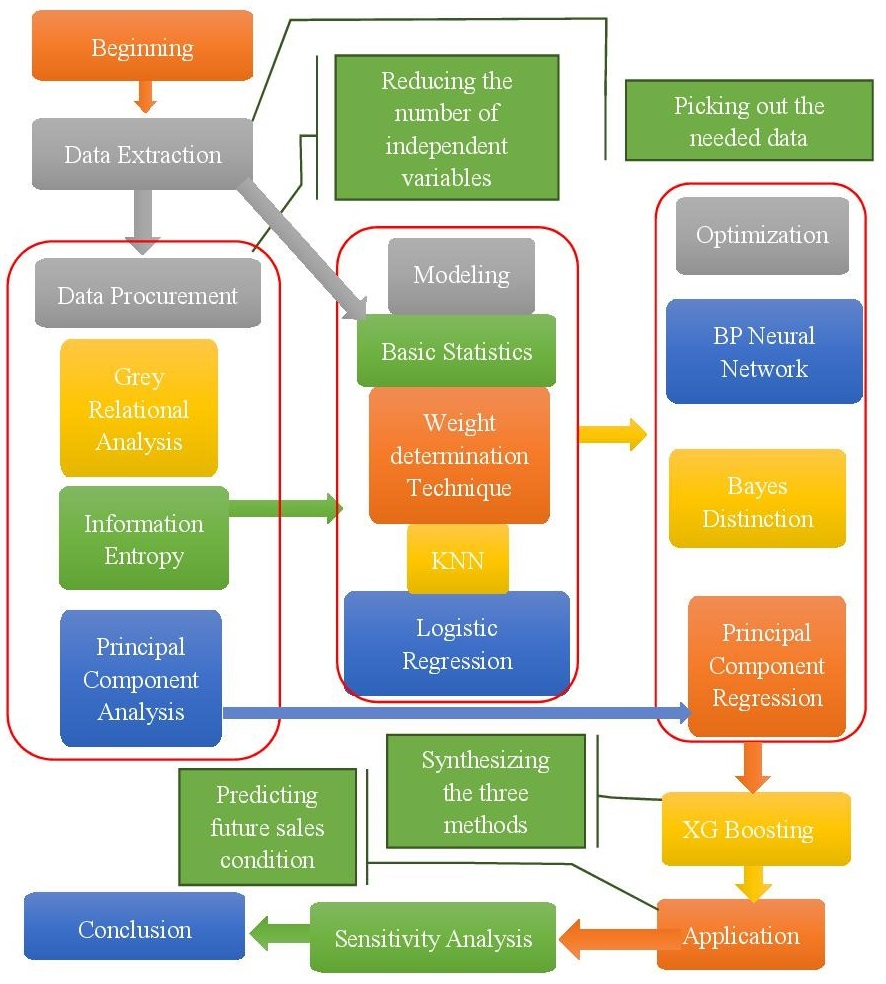
\includegraphics[width=15.00cm]{1.jpg}\\
  \caption{The flow chart of the whole modeling process}\label{fig1}
\end{figure}


Figure \ref{fig1} above presents the whole modeling process. In order to solve the problem illustrated above, we consider to divide the whole process into several parts. To predict sales conditions of new phones, we need to study sales conditions of existing phones. As the real situation is too complex and complicated, we need to make several reasonable assumptions to simplify the real-world implications without the loss of the core. As the raw data from products sold in AliExpress cannot be used straightly for modeling, we need to extract useful and relevant data. In light of the vast amount of data which costs too much time to analyze without apparent benefits, we need to decide most influential factors for further analysis, which is the data procurement part, to reduce the number of independent factors. In this process, we apply three different methods: Grey Relational Analysis, Principal Component Analysis, and Information Entropy. The Grey Relational Analysis fails to reduce the number of influential factors, while the other two methods effectively achieve the goal. Then we apply the results of data procurement for modeling. In the modeling process, we apply results from Principal Component Analysis to Weight Determination Technique, KNN, and Logistic Regression. At this point, although we have reached conclusions of the rank of different independent factors, none of them is satisfactory enough, which brings out the optimization for each model. We employ Principal Component Regression, Bayes Distinction, and BP Neural Network Fitting to optimize the model, while all of them feature advantages and drawbacks. Hence, we employ the XG Boosting algorithm to synthesize the three methods and reach the most accurate conclusion about which characteristics contribute to the highest sale volume. We apply our research results on predicting future sales conditions. Finally, we do the sensitivity analysis to show that our model is robust.

\section{Assumptions, Justifications, and Definitions}

\subsection{Assumptions and Justifications}

\textbf{We make the following assumptions in order to simplify the model without much loss of the core of the problem. We also include a justification part to show that our assumptions are reasonable.}

\begin{itemize}
	\item Assumption 1: We assume that considering Category Click and Convert rate as the bases for the Information Gain provide authentic information and reflect the ratio of people who are interested in and actually buy the cell phone.
	
	Justification: the data are also in a more consistent and standardized form which is convenient for later grouping and processing.
\end{itemize}



\begin{itemize}
	\item Assumption 2: All the data which pass the data process and procurement part are credible and reliable, meaning that they have no error.

Justification: In light of the fact that the data are provided by AliExpress, which comes from reliable sources, the data ought to be without fabrication.
\end{itemize}

\begin{itemize}
	\item Assumption 3: Except the parameters given in the data, all other factors, including but not limited to the other properties of the cell phones, such as the advertisement of the cell phones propagated by the manufacturer, are exactly the same, which indicates that it has no impact of difference on the click rate and the convert rate between each phone.

Justification: We make the assumption to simplify the problem, while we are unable to find and evaluate the data of the cell phones other than the given ones.
\end{itemize}

\begin{itemize}
	\item Assumption 4: All the cell phones are suitable for customers to use, which means all the coasters have no potential safety hazards, and the coasters will not physically and/or mentally harm the users. For instance, the light generated by the screens will not harm the eyes of the users.

Justification: In accordance with the local policies and the regulations, all the cell phones in the market ought to have passed the mandatory security test given by local authorities, which institute the rules to eradicate safety concerns.

\end{itemize}
\subsection{Definitions}

\textbf{Here we clarify the definitions of the key terms we are going to use and the notations we will employ to expand the mathematical derivation.}

\begin{itemize}
	\item \textbf{Convert Rate} represents the ratio of the number of people who buy that certain type of cell phone to the number of people who click on the picture online for more detail.

\end{itemize}
\begin{itemize}
	\item \textbf{Click Rate} represents the ratio of the number of people who click on the picture for more detail to the number of people who browse the internet and see the picture of that certain type of cell phone.
\end{itemize}


The following table \ref{Notation1}-\ref{Notation3} shows the definitions in the paper.

\begin{table}
  \centering
  \begin{tabular}{|l|l|}
\hline
\multicolumn{1}{|c|}{Notation}                                         & Definition                                                                                                                                                                                    \\ \hline
$A_{ij}$                                                                 & \begin{tabular}[c]{@{}l@{}}The element in $i^{th}$ row and $j^{th}$ column in matrix $A$\end{tabular}                                                                                         \\ \hline
$X$                                                                    & \begin{tabular}[c]{@{}l@{}}The independent variables matrix\end{tabular}                                                                                                                  \\ \hline
$x$                                                                    & \begin{tabular}[c]{@{}l@{}}Row vector of independent variables\end{tabular}                                                                                                               \\ \hline
$y$                                                                    & \begin{tabular}[c]{@{}l@{}}Row vector of dependent variables\end{tabular}                                                                                                                 \\ \hline
$\overline{x}$                                        & \begin{tabular}[c]{@{}l@{}}The algebra average of several data\end{tabular}                                                                                                               \\ \hline
$Y_1$                                                                  & \begin{tabular}[c]{@{}l@{}}Click rate sequence in Grey Relational Analysis or click rate matrix\\ in other parts\end{tabular}                                                               \\ \hline
$Y_2$                                                                  & \begin{tabular}[c]{@{}l@{}}Convert rate sequence in Grey Relational Analysis or convert rate matrix\\ in other parts\end{tabular}                                                           \\ \hline
$X_k$                                                                  & \begin{tabular}[c]{@{}l@{}}The $k^{th}$ independent variable sequence in Grey Relational Analysis\end{tabular}                                                               \\ \hline
$Y_k^n$                                                                  & \begin{tabular}[c]{@{}l@{}}The $n^{th}$ number in the $k^{th}$ dependent variable sequence\\ in Grey Relational Analysis\end{tabular}                             \\ \hline
$X_k^n$                                                                & \begin{tabular}[c]{@{}l@{}}The $n^{th}$ number in the $k^{th}$ independent variable sequence in\\ Grey Relational Analysis\end{tabular}                           \\ \hline
\begin{tabular}[c]{@{}l@{}}$\Delta X_k^n$\end{tabular}             & \begin{tabular}[c]{@{}l@{}}The difference between every two adjacent terms in independent variable\\ sequences in Grey Relational Analysis\end{tabular}                                 \\ \hline
\begin{tabular}[c]{@{}l@{}}$\Delta   Y_k^n$\end{tabular}             & \begin{tabular}[c]{@{}l@{}}The difference between every two adjacent terms in dependent variable\\ sequences in Grey Relational Analysis\end{tabular}                                   \\ \hline
$CC(Y_k)$                                                              & \begin{tabular}[c]{@{}l@{}}The correlation coefficient of $k^{th}$ dependent variable sequence\end{tabular}                                                                  \\ \hline
$CC(Y_k,X_l)$                                                          & \begin{tabular}[c]{@{}l@{}}The correlation coefficient between $k^{th}$ dependent variable sequence and\\ $l^{th}$ independent variable sequence\end{tabular} \\ \hline
$\gamma(Y_k,X_l)$                                                      & \begin{tabular}[c]{@{}l@{}}The correlation degree between the $k^{th}$ dependent variable sequence and\\ $l^{th}$ independent variable sequence\end{tabular}  \\ \hline
$E(X)$                                                                 & \begin{tabular}[c]{@{}l@{}}The information entropy regarding the set of incidence $X$\end{tabular}                                                                                          \\ \hline
$P_i$                                                                  & \begin{tabular}[c]{@{}l@{}}The probability that incident numbered $i$ will happen in the set $X$\end{tabular}                                                                                 \\ \hline
$E(global)$                                                            & \begin{tabular}[c]{@{}l@{}}The information entropy of Category Click and Convert Rate\end{tabular}                                                                                        \\ \hline
$IGain$                                                                & \begin{tabular}[c]{@{}l@{}}The information gain of individual variables related to\\ the Category Click and Convert Rate\end{tabular}                                                      \\ \hline
\end{tabular}
  \caption{The definition of notations-1}\label{Notation1}
\end{table}

\begin{table}
  \centering
  \begin{tabular}{|l|l|}
\hline
\multicolumn{1}{|c|}{Notation}                                         & Definition                                                                                                                                                                                    \\ \hline
$A_{i,j}$                                                                & \begin{tabular}[c]{@{}l@{}}The data in the $i^{th}$ line and $j^{th}$ column in the table of data processing\\ concerning information entropy\end{tabular}    \\ \hline
$x_p$                                                                       & \begin{tabular}[c]{@{}l@{}}The $p^{th}$ original variable\end{tabular}                                                                                                       \\ \hline
$z_q$                                                                  & \begin{tabular}[c]{@{}l@{}}The $q{th}$ npew variable\end{tabular}                                                                                                            \\ \hline
$m$                                                                    & \begin{tabular}[c]{@{}l@{}}The number of samples\end{tabular}                                                                                                                             \\ \hline
$l$                                                                    & \begin{tabular}[c]{@{}l@{}}The number of variables in each sample\end{tabular}                                                                                                            \\ \hline
$x_{ij}$                                                                 & \begin{tabular}[c]{@{}l@{}}The standardized data at row $i$ and column $j$\end{tabular}                                                                                                       \\ \hline
$x_{ij}^*$                                                               & \begin{tabular}[c]{@{}l@{}}The data at row $i$ and column $j$ before standardization\end{tabular}                                                                                             \\ \hline
$R$                                                                    & \begin{tabular}[c]{@{}l@{}}The correlation coefficient matrix in principal component analysis\end{tabular}                                                                                \\ \hline
$\lambda_q$                                                            & \begin{tabular}[c]{@{}l@{}}The $q^{th}$ characteristic roots or eigenvalues in weight\\   determination technique\end{tabular}                                               \\ \hline
$a_q(A_q)$                                                             & \begin{tabular}[c]{@{}l@{}}The $q^{th}$ characteristic vectors\end{tabular}                                                                                                  \\ \hline
$a_{pq}$                                                                 & \begin{tabular}[c]{@{}l@{}}The $p^{th}$ value of the $q^{th}$ characteristic vectors\end{tabular}                                                                                \\ \hline
$(w_1,��,w_n)$                                                          & \begin{tabular}[c]{@{}l@{}}Weight vector in Weight Determination Technique\end{tabular}                                                                                                   \\ \hline
$n$                                                                    & \begin{tabular}[c]{@{}l@{}}The number of choices of target layer in Weight Determination Technique\end{tabular}                                                                           \\ \hline
$w$                                                                    & \begin{tabular}[c]{@{}l@{}}The eigenvector in Weight Determination Technique\end{tabular}                                                                                                 \\ \hline
$\beta$                                                                & \begin{tabular}[c]{@{}l@{}}Coefficient matrixes of the original data\end{tabular}                                                                                                         \\ \hline
$\beta'$                                                              & \begin{tabular}[c]{@{}l@{}}Coefficient matrixes of Principal Component Regression\end{tabular}                                                                                            \\ \hline
$P\{X\}$                                                                 & \begin{tabular}[c]{@{}l@{}}The probability that satisfies condition $X$\end{tabular}                                                                                                        \\ \hline
$\alpha$                                                               & \begin{tabular}[c]{@{}l@{}}Reliability in Regression\end{tabular}                                                                                                                         \\ \hline
$\theta$                                                               & \begin{tabular}[c]{@{}l@{}}Parameters to be estimated of the ensemble in Regression\end{tabular}                                                                                          \\ \hline
$\hat{\theta_1}$                                                       & \begin{tabular}[c]{@{}l@{}}The confidence upper limit in Regression\end{tabular}                                                                                                          \\ \hline
$\hat{\theta_2}$                                                       & \begin{tabular}[c]{@{}l@{}}The confidence lower limit in Regression\end{tabular}                                                                                                          \\ \hline
$d(X,Y)$                                                               & \begin{tabular}[c]{@{}l@{}}The Mahalanobis distance of the data\end{tabular}                                                                                                              \\ \hline
$\Omega$                                                               & \begin{tabular}[c]{@{}l@{}}The covariance matrix\end{tabular}
\\ \hline
\end{tabular}
  \caption{The definition of notations-2}\label{Notation2}
\end{table}
\begin{table}
  \centering
  \begin{tabular}{|l|l|}
\hline
\multicolumn{1}{|c|}{Notation}                                         & Definition                                                                                                                                                                                    \\ \hline
\begin{tabular}[c]{@{}l@{}}$P(B_i|A)$\end{tabular} & \begin{tabular}[c]{@{}l@{}}Posteriori probability in Bayes Distinction\end{tabular}                                                                                                       \\ \hline
\begin{tabular}[c]{@{}l@{}}$P(A|B_i)$\end{tabular} & \begin{tabular}[c]{@{}l@{}}Priori probability in Bayes Distinction\end{tabular}                                                                                                           \\ \hline
$P(B_i)$                                                               & \begin{tabular}[c]{@{}l@{}}The frequency at which the sample appears in Bayes Distinction\end{tabular}                                                                                    \\ \hline
$G_i$                                                                  & \begin{tabular}[c]{@{}l@{}}The ensemble in Bayes Distinction\end{tabular}                                                                                                                 \\ \hline
$f(x)$                                                                 & \begin{tabular}[c]{@{}l@{}}Probability density function of $G_i$ in Bayes Distinction\end{tabular}                                                                                         \\ \hline
$p_i$                                                                  & \begin{tabular}[c]{@{}l@{}}The priori probability of $G_i$ in Bayes Distinction\end{tabular}                                                                                               \\ \hline
$k$                                                                    & \begin{tabular}[c]{@{}l@{}}The number of $G_i$ in Bayes Distinction\end{tabular}                                                                                                           \\ \hline
$P(\frac{j}{i})$                                                       & \begin{tabular}[c]{@{}l@{}}The conditional probability of wrongly categorizing the sample of $G_i$\\ to the ensemble $G_j$\end{tabular}                                                       \\ \hline
$C(\frac{j}{i})$                                                       & \begin{tabular}[c]{@{}l@{}}The loss caused by the wrong categorization\end{tabular}                                                                                                       \\ \hline
$D_k$                                                                  & \begin{tabular}[c]{@{}l@{}}A division of a set of distinction samples\end{tabular}                                                                                                        \\ \hline
$ECM$                                                                  & \begin{tabular}[c]{@{}l@{}}The average wrong distinction loss\end{tabular}                                                                                                                \\ \hline
$L(\theta)$                                                            & \begin{tabular}[c]{@{}l@{}}The overall loss of each classifier\end{tabular}                                                                                                               \\ \hline
$y_i$                                                                  & \begin{tabular}[c]{@{}l@{}}Classification function\end{tabular}                                                                                                                           \\ \hline
$\hat{y_i}$                                                            & \begin{tabular}[c]{@{}l@{}}function of each classifier to reduce the loss\end{tabular}                                                                                                    \\ \hline
$S_k$                                                                  & \begin{tabular}[c]{@{}l@{}}The score of the data to show the accuracy of the prediction\end{tabular}                                                                                      \\ \hline
\end{tabular}
  \caption{The definition of notations-3}\label{Notation3}
\end{table}


\section{Data Procurement and Process}

\textbf{As the raw data from products sold in AliExpress cannot be used straightly for modeling, we need to extract useful and relevant data. In light of the vast amount of data which costs too much time to analyze without apparent benefits, we need to decide different influential factors for further analysis to reduce the number of independent factors.}

\subsection{Data extraction}

We have obtained information about sale records on AliExpress, which is under the control of Alibaba. The original data is in the appendix. With the algorithm and formula given by AliExpress, we convert the original data into the readable and understandable data, which can also be seen in the appendix. [11][12]

We utilize PYTHON to extract the parameter cells, which contain several standardized descriptions of the phones. With the help of XLRD module and XLWR module, we search for cells with the assigned field one after another. We divide the searching process into two stages. The first stage is to separate the entire parameters into several fields that contain only one property each; The second stage is to check what each field denotes and use numerical data to characterize the words. For instance, when we search for the battery property, which is detachable, not detachable, or unknown, we first split the cell by ``$<$br$>$" which stands for breaks to obtain strings that merely possess one property in lieu of many.

Then we use the ``if" function to determine whether the obtained string includes target string, which is ``yes" or ``no" standing for detachable or not detachable. If it includes the prior one, we define the corresponding value in the new Excel table as 1. If it includes the latter one, we define the corresponding value in the new Excel table as 2. If it includes neither one, we define the corresponding value in the new Excel table as 0, which stands for unknown.

We set Unlock Phones, Google Play, Battery Type, Display Resolution, Operation System, Gravity Response, GPRS, SIM Card Quantity, Size, Battery Capacity, Camera, Recording Definition, Display Size, Brand Name, CPU, Touch Screen Type, RAM, and ROM as the keywords for the first stage; we set ``yes" and ``no" as the keywords for the second stage.

In the second stage, there are some individual cases for us to pay attention to. When we extract the color parameters, we search the name of the colors individually, for the reason that a page may contain phones with various colors. We use the binary combinations to express the colors of the phones. We set White, Blue, Rose, Gold, Silver, Grey, Pink, Brown, Orange, Yellow, and Red as the detection keywords, which allows us to obtain eleven-dimensional binary array to demonstrate the colors. The following figure \ref{fig2} illustrates the process.

\begin{figure}
  %\centering
  % Requires \usepackage{graphicx}
  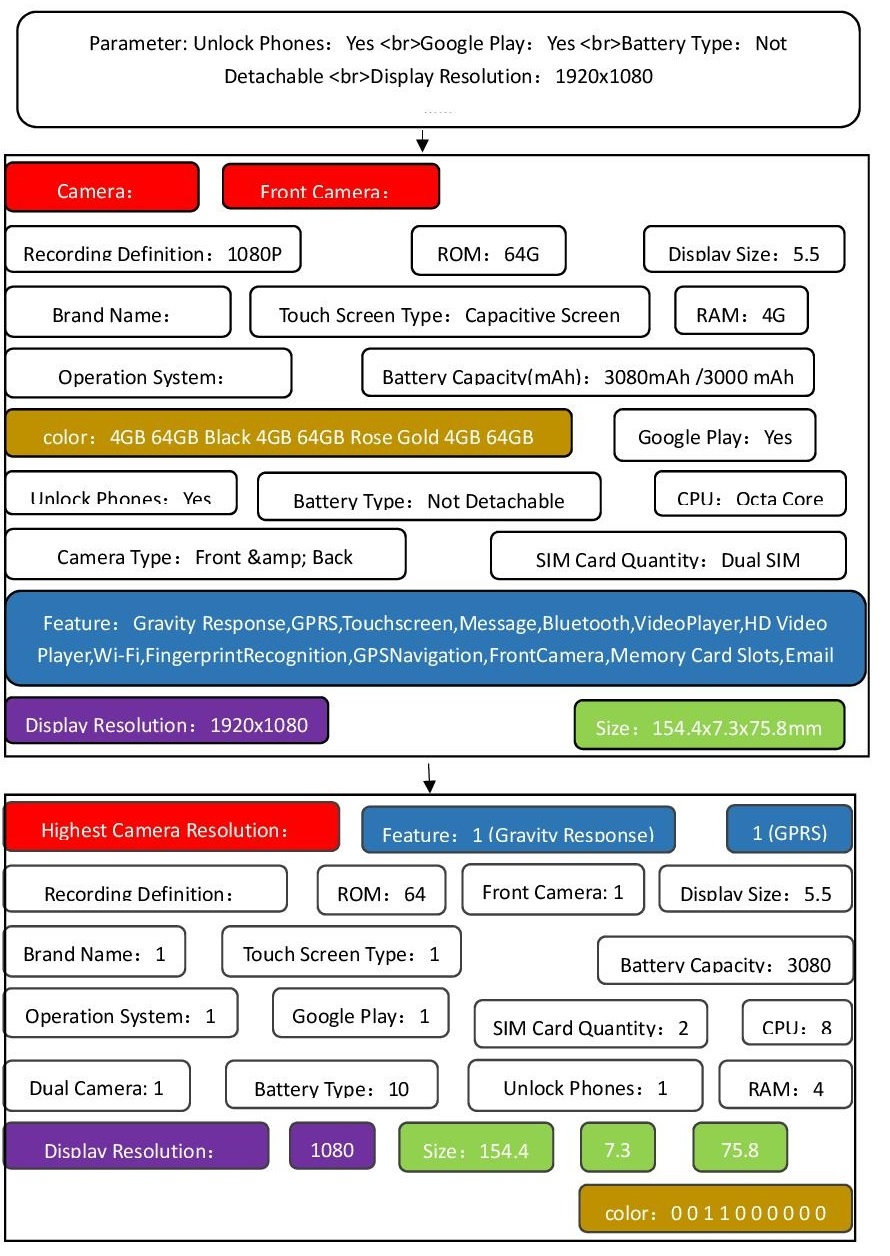
\includegraphics[width=15.00cm]{2.jpg}\\
  \caption{Data Extraction diagram}\label{fig2}
\end{figure}
When we are extracting the highest camera resolution fields, we search all the fields with ``camera:" and comparing the numerical part of all the fields featuring above, retaining the largest one and disposing of the rest.

As for extracting the size, we encounter a problem that some of the dimensions are expressed in inches, while others are in centimeters or millimeters, triggering inconsistency in units. To solve this issue, we first use ``x" or ``*" to split the value of three dimensions, before we multiply the three parameters, get the volume of the phones, and use a method to determine the critical value that decides the unit of the phones. We select a phone that we regard as normal, calculating the volume among in inches, millimeters, and centimeters. We then obtain the square roots of the size in inches and centimeters, as well as in centimeters and in millimeters, which are regarded as the critical value. We obtain the essential values of volume, which are 36.86334 and 4712.451. If the product is less than 36.86334, we associate the unit as inches. Then we multiply the length, width, and height of the phone with 25.4 to obtain the corresponding value in millimeters. If the product is more than 36.86334 but less than 4712.451, we regard the unit as centimeters. Then we multiply the length, width, and height of the phone with 10 to obtain the corresponding value in millimeters. If the product is more than 4712.451, we regard the unit as millimeters. Then we straight write the length, width, and height of the phone into the tables.

Finally, we write the value into the Excel table and obtain the data we use, which can be seen in the appendix.

\subsection{Grey Relational Analysis}

In the real world, it is commonly seen that a system tends to be influenced by multi-factors instead of a single one, and the relationship between factors is complicated. Therefore, it is easy to cover up the system��s essence with mere regards of its appearance, which makes it difficult to get accurate information and distinguish the primary and secondary factors. \textbf{The grey system analysis method is essentially an analytic method that replaces discrete data with linked concepts and define the importance between each label. [8]}

The grey system theory holds that, although the appearance of the objective system seems to be complicated, and the data is irrelevant, it always functions as a whole, which means it is not random but proves to contain some inherent laws that can be discovered and explored, and the key is how to choose the proper way to figure out the rules of the data and utilize them.

The gray correlation degree is calculated as follows in general: first, we standardize the collected evaluation data to ensure that it is treated without dimension; we obtain the sequence of difference and compute the maximum and minimum variance of the series of difference; we calculate the correlation coefficient and the calculation correlation degree.

Specifically, we consider the dependent variables, which are click rate and conversion rate, as the reference sequence. As shown in the appendix, we let the following sequence \ref{for1} denotes the click rate sequence:

\begin{equation}\label{for1}
Y _ { 1 } = Y _ { 1 } ^ { 1 } , Y _ { 1 } ^ { 2 } , Y _ { 1 } ^ { 3 } , Y _ { 1 } ^ { 4 } , \ldots , Y _ { 1 } ^ { 1324 }
\end{equation}

And we let the following sequence \ref{for2} as the convert rate sequence:

\begin{equation}\label{for2}
Y _ { 2 } = Y _ { 2 } ^ { 1 } , Y _ { 2 } ^ { 2 } , Y _ { 2 } ^ { 3 } , Y _ { 2 } ^ { 4 } , \ldots , Y _ { 2 } ^ { 1324 }
\end{equation}

We consider the 26 series of independent variables as comparing sequence. As shown in the appendix, we let the following sequence \ref{for3} denote the Google play sequence:

\begin{equation}\label{for3}
X _ { 1 } = X _ { 1 } ^ { 1 } , X _ { 1 } ^ { 2 } , X _ { 1 } ^ { 3 } , X _ { 1 } ^ { 4 } , \ldots , X _ { 1 } ^ { 1324 }
\end{equation}
	
	Then, we let the following sequence \ref{for4} be the can-design-product sequence:
	
	\begin{equation}\label{for4}
	X _ { 26 } = X _ { 26 } ^ { 1 } , X _ { 26 } ^ { 2 } , X _ { 26 } ^ { 3 } , X _ { 26 } ^ { 4 } , \ldots , X _ { 26 } ^ { 1324 }
	\end{equation}
	
	Then we standardize the data, making the variance of each sequence change into 1 and the mean into 0. We compute the difference between every two adjacent terms, which can be shown as following formula \ref{for5}-\ref{for6}:
	

	\begin{equation}\label{for5}
    \begin{aligned}
    \Delta X _ { k } ^ { n } & = X _ { k } ^ { n + 1 } - X _ { k } ^ { n } \left( k \epsilon \left\{ k \in \mathbb { N } ^ { * } | k \leq 26 \right\} , n \epsilon \left\{ n \in \mathbb { N } ^ { * } | n \leq 1323 \right\} \right)
    \end{aligned}
	\end{equation}
    \begin{equation}\label{for6}
    \begin{aligned}
    \Delta Y _ { k } ^ { n } & = Y _ { k } ^ { n + 1 } - Y _ { k } ^ { n } \left( k \epsilon \left\{ k \in \mathbb { N } ^ { * } | k \leq 2 \right\} , n \epsilon \left\{ n \in \mathbb { N } ^ { * } | n \leq 1323 \right\} \right)
    \end{aligned}
	\end{equation}

	

	We finally calculate correlation coefficients and the correlation degree, as in formula \ref{for7}-\ref{for9}. The result of Grey Relational Analysis is shown in table \ref{Grey Relational Analysis Result}.


\begin{table}[]
\centering
\begin{tabular}{|l|l|l|l|l}
\cline{1-4}
\multicolumn{1}{|c|}{} & Google Play                                                              & Battery Type      & \begin{tabular}[c]{@{}l@{}}Battery\\   Capacity(mAh)\end{tabular} &                               \\ \cline{1-4}
Click Rate             & 0.958033                                                                 & 0.958033          & 0.54663                                                           &                               \\ \cline{1-4}
Convert Rate           & 0.989033                                                                 & 0.989033          & 0.563529                                                          &                               \\ \cline{1-4}
                       & \begin{tabular}[c]{@{}l@{}}Recording \\ Definition (P)\end{tabular}      & Touch Screen Type & RAM(G)                                                            &                               \\ \cline{1-4}
Click Rate             & 0.958033                                                                 & 0.958033          & 0.588991                                                          &                               \\ \cline{1-4}
Convert Rate           & 0.989033                                                                 & 0.989033          & 0.570534                                                          &                               \\ \cline{1-4}
                       & \begin{tabular}[c]{@{}l@{}}Highest camera \\ resolution(MB)\end{tabular} & Dual Camera       & Front Camera                                                      &                               \\ \cline{1-4}
Click Rate             & 0.771525                                                                 & 0.958033          & 0.958033                                                          &                               \\ \cline{1-4}
Convert Rate           & 0.805639                                                                 & 0.989033          & 0.989033                                                          &                               \\ \cline{1-4}
                       & SearchCnt                                                                & GoodCommentCount  & Score                                                             &                               \\ \cline{1-4}
Click Rate             & 0.752451                                                                 & 0.550346          & 0.958033                                                          &                               \\ \cline{1-4}
Convert Rate           & 0.722596                                                                 & 0.56748           & 0.989033                                                          &                               \\ \cline{1-4}
                       & Display Resolution                                                       & Operation System  & SIM Card Quantity                                                 &                               \\ \cline{1-4}
Click Rate             & 0.958033                                                                 & 0.958033          & 0.958033                                                          &                               \\ \cline{1-4}
Convert Rate           & 0.989033                                                                 & 0.989033          & 0.989033                                                          &                               \\ \hline
                       & ROM(G)                                                                   & CPU               & Display Size (inches)                                             & \multicolumn{1}{l|}{Size}     \\ \hline
Click Rate             & 0.337011                                                                 & 0.958033          & 0.958033                                                          & \multicolumn{1}{l|}{0.771116} \\ \hline
Convert Rate           & 0.330881                                                                 & 0.989033          & 0.989033                                                          & \multicolumn{1}{l|}{0.805193} \\ \hline
                       & Brand                                                                    & Color             & Feature                                                           & \multicolumn{1}{l|}{Price}    \\ \hline
Click Rate             & 0.958033                                                                 & 0.486192          & 0.958033                                                          & \multicolumn{1}{l|}{0.555845} \\ \hline
Convert Rate           & 0.989033                                                                 & 0.499513          & 0.989033                                                          & \multicolumn{1}{l|}{0.539377} \\ \hline
                       & IsGalleryFeatured                                                        & IsHighQuality     & CanDesignProduct                                                  &                               \\ \cline{1-4}
Click Rate             & 0.958033                                                                 & 0.958033          & 0.958033                                                          &                               \\ \cline{1-4}
Convert Rate           & 0.989033                                                                 & 0.989033          & 0.989033                                                          &                               \\ \cline{1-4}
\end{tabular}

\caption{Grey Relational Analysis Result}\label{Grey Relational Analysis Result}
\end{table}
	
	\begin{equation}\label{for7}
	{ C C \left( Y _ { k } \right) = \left| \sum _ { i = 1 } ^ { 1323 } \frac { \Delta Y _ { k } ^ { i } } { n } \right| \left( k \epsilon \left\{ k \in \mathbb { N } ^ { * } | k \leq 2 \right\} \right) }
 \end{equation}
 \begin{equation}\label{for8}
 { C C \left( Y _ { k } , X _ { l } \right) = \left| \sum _ { i = 1 } ^ { 1323 } \frac { \Delta Y _ { k } ^ { i } - \Delta X _ { l } ^ { i } } { n } \right| \left( k \epsilon \left\{ k \in \mathbb { N } ^ { * } | k \leq 2 \right\} , l \epsilon \left\{ l \in \mathbb { N } ^ { * } | l \leq 26 \right\} \right) }
  \end{equation}
  \begin{equation}\label{for9}
  { \gamma \left( Y _ { k } , X _ { l } \right) = \frac { 1 + C C \left( Y _ { k } \right) } { 1 + C C \left( Y _ { k } \right) + C C \left( Y _ { k } , X _ { l } \right) } \left( k \epsilon \left\{ k \in \mathbb { N } ^ { * } | k \leq 2 \right\} , l \epsilon \left\{ l \in \mathbb { N } ^ { * } | l \leq 26 \right\} \right) }
	\end{equation}
	
	From the obtained correlation degree in table 2, we find that the independent variables which have less value in them are apt to have higher correlation values, symbolizing that a closer connection with the dependent variables. Moreover, the independent variables which have the same number of value possess the same correlation degree, rendering it impossible for us to distinguish how close the connections are between these independent variables and the target dependent variables. \textbf{We can conclude that the Grey Relational Analysis suits for continuous variables rather than discrete variables, indicating that it is not an ideal technique for us to determine how strong the relationship is under this situation.} It does not mean that the models in red do not work well for the problems; it merely means that this model is technically correct and work if the data are all continuous, while they are not perfectly suitable for the current data given.
	
	\subsection{Information Entropy}
	
	Information entropy is defined by the formula \ref{for10} below:
	
	\begin{equation}\label{for10}
	E ( X ) = - \sum _ { i = 1 } ^ { n } p _ { i } \log _ { 2 } \left( p _ { i } \right)
	\end{equation}
	
	where $E ( X )$ represents the Information Entropy of $X$, the set of incidents taken into consideration (in the formula 10 the total number of incidents is $n$), and $p _ { i }$ represents the possibility that the incident numbered $i$ will happen in the set $X_p$. The information entropy is calculated in the form of the sum of each individual incident.
	
\textbf{Information entropy is used to reflect the complexity of the information being processed. Higher information entropy value indicates a higher degree of information complexity. Thus, information entropy can be applied to analyze the information in a quantitative way.}

However, in determining which factor is more important for us to take into consideration among the 26 individual variables related to the cell phone as extracted, what is needed should be the amount of information that can be acquired from analyzing on factor instead of its complexity as reflected by the information entropy. Therefore, we utilize information gain to consider which factors are the top ones that should be taken into account as the most crucial. In other words, what kinds of factors contribute more or promote the sale of the smartphones in general. The calculation of information gain of each factor involves its information entropy and is a deliberate and complex process. In the next part of this section, we will mainly discuss the data processing related to the information gain.

First, we identify 26 individual variables as the potentially influential factors for sale volume of cell phones including Google play, battery type, brand, RAM, ROM, dual camera, front camera, display size, etc. Then, types of data representing the actual sale volume of cellphones are regarded as the bases for calculating the information gain. Instead of choosing the actual sales volume, we consider the Category Click Rate and Category Convert Rate. Reasons are given in the assumption.

We then divide the Category Click Rate and Category Convert Rate into five groups respectively and reasonably, according to the individual value of the data, from high to low, categorized from 1 to 5. After categorizing the data related to Category Click and Convert Rate, we use formula 10 to calculate the global information entropy of those two sets respectively. As applying the formula to the Category Click Rate, $E(X)$ now represents the information entropy of the Category Click Rate, and $p _ { i }$ represents the possibility of category numbered $i$ will happen. Especially, since there are 5 categories, the number $n$ equals 5. The same can be applied to the Category Convert Rate, and the final results are shown in table \ref{The Global information entropy}.
\begin{table}
  \centering
  \begin{tabular}{|l|l|l|}
\hline
\multicolumn{1}{|c|}{}               & \begin{tabular}[c]{@{}l@{}}Category Click\\   Rate\end{tabular} & \begin{tabular}[c]{@{}l@{}}Category Convert\\   Rate\end{tabular} \\ \hline
Global information entropy $E(global)$ & 2.200779                                                        & 2.081891                                                          \\ \hline
\end{tabular}
  \caption{The Global information entropy}\label{The Global information entropy}
\end{table}

The information we can get from each individual variable is calculated respectively, and the individual variables can be generally classified into two groups: group one with relevant data presenting in inconsistent ways, including factors like Is Gallery Featured and Dual Camera, in which the data only consist of 1, 0, or -1(in other words, the data are expressed in simple forms and can be calculated manually); group two with relevant data presenting in consistent forms, including factors like Display Size and Display Resolution, in which the data are in various forms and need grouping for further calculation.

As for group one, we take ROM as an example to illustrate how the information entropy is calculated based on the grouping of Category Click Rate. First, we do the grouping and data processing. The data of ROM are presented as discrete variables, including 2, 4, 8, 16, 32, 64, 128, and 256. The grouping of data in ROM should also be related to the grouping of Category Click Rate, so accordingly, there are in total 40 groups, which are presented in table \ref{ROM to Category Click Rate}.

\begin{table}
  \centering
  \begin{tabular}{|l|l|l|l|l|l|l|}
\hline
\multicolumn{1}{|c|}{ROM} & \begin{tabular}[c]{@{}l@{}}Group number in\\   Category Click Rate\end{tabular} & 1   & 2  & 3   & 4   & 5  \\ \hline
                          & 2                                                                               & 0   & 3  & 2   & 1   & 0  \\ \hline
                          & 4                                                                               & 5   & 6  & 13  & 7   & 0  \\ \hline
                          & 8                                                                               & 64  & 38 & 63  & 54  & 8  \\ \hline
                          & 16                                                                              & 110 & 89 & 132 & 143 & 36 \\ \hline
                          & 32                                                                              & 64  & 44 & 82  & 63  & 29 \\ \hline
                          & 64                                                                              & 83  & 38 & 62  & 49  & 16 \\ \hline
                          & 128                                                                             & 3   & 4  & 5   & 7   & 0  \\ \hline
                          & 256                                                                             & 0   & 0  & 1   & 0   & 0  \\ \hline
\end{tabular}
  \caption{The grouping of ROM related to Category Click Rate}\label{ROM to Category Click Rate}
\end{table}

Let $i$ represents the $i ^ { t h }$ line in the table of the forty groups, $j$ represents the $j ^ { t h }$ column in the table, and $A _ { i j }$ represents the number in the unit of the  $i ^ { t h }$ line and $j ^ { t h }$ column. Thus, in the unit $A _ { 4,1 }$, the number 110 represents that there are in total 110 data in ROM that are 16 and also in the group 1 as categorized according to the Category Click Rate. Notice that the sum of all the forty groups should equal to the total number of data (and in our data processing, the total number of data available is 1324).

After the grouping of ROM data related to the Category Click Rate, we further calculate the information entropy of the data in each line using formula \ref{for10}. The information entropy of ROM in each line is shown in table \ref{Information entropy of ROM}.

\begin{table}
  \centering
  \begin{tabular}{|l|l|l|l|l|l|}
\hline
\multicolumn{1}{|c|}{} &    &     &     &    & Information entropy \emph{E(ROM)} \\ \hline
0                      & 3  & 2   & 1   & 0  & 1.459148            \\ \hline
5                      & 6  & 13  & 7   & 0  & 1.89366             \\ \hline
64                     & 38 & 63  & 54  & 8  & 2.122787            \\ \hline
110                    & 89 & 132 & 143 & 36 & 2.205866            \\ \hline
64                     & 44 & 82  & 63  & 29 & 2.242444            \\ \hline
83                     & 38 & 62  & 49  & 16 & 2.160525            \\ \hline
3                      & 4  & 5   & 7   & 0  & 1.931295            \\ \hline
0                      & 0  & 1   & 0   & 0  & 0                   \\ \hline
\end{tabular}
  \caption{Information entropy of ROM}\label{Information entropy of ROM}
\end{table}


In order to acquire the total amount of information we can gain from the independent variable ROM, we need to further calculate the probability that each line will happen. As for the first line $A_{(1,j)}$, we calculate the times at which data 2 appears and then divide the total number of data, 1324. Then, we multiply the probability to the information entropy of each line, the results are shown in table \ref{The Information entropy}.

\begin{table}
  \centering
  \begin{tabular}{|l|l|l|}
\hline
\multicolumn{1}{|c|}{Information entropy} & Probability & Product  \\ \hline
1.459148                                  & 0.004532    & 0.006612 \\ \hline
1.89366                                   & 0.023414    & 0.044338 \\ \hline
2.122787                                  & 0.17145     & 0.363952 \\ \hline
2.205866                                  & 0.385196    & 0.849692 \\ \hline
2.242444                                  & 0.212991    & 0.47762  \\ \hline
2.160525                                  & 0.187311    & 0.40469  \\ \hline
1.931295                                  & 0.01435     & 0.027715 \\ \hline
0                                         & 0.000755    & 0        \\ \hline
\end{tabular}
  \caption{The Information entropy, possibility and their products of ROM}\label{The Information entropy}
\end{table}

The sum of all eight products is the total information entropy we can get from the individual variable ROM. However, for the information gain as related to the
Category Click Rate, we need to use the global information entropy of Category Click Rate to subtract the sum of the product above, as the following formula \ref{for11} presents:

\begin{equation}\label{for11}
{  { IGain(Category Click Rate, Rom) } }  { = E (  {global} ) - \sum  { Information entropy } \times  { Possibility } }
\end{equation}

where $E(global)$ here represents the global information entropy of the Category Click Rate, since the gain is related to the Category Click Rate. The final gain is presented in table \ref{final information gain ROM}.

\begin{table}
  \centering
  \begin{tabular}{|l|l|l|}
\hline
\multicolumn{1}{|c|}{} & \begin{tabular}[c]{@{}l@{}}Sum of the products\end{tabular} & \emph{IGain}        \\ \hline
ROM                    & 2.17462                                                         & 0.026159 \\ \hline
\end{tabular}
  \caption{The final information gain of ROM}\label{final information gain ROM}
\end{table}

Similarly, the information gain of ROM related to the Category Convert Rate can also be calculated using the method above, and the only difference will be the data in the 40 groups and in the final formula, $E(global)$p should represent the global information entropy of the Category Convert Rate.

As for the group two, we consider the Search Count (the number of time that a certain type of phone is exposed to the customer) as related to the Category Click Rate in order to illustrate the difference of data processing from group one. From the data we have extracted, it is obvious that the data in the Search Count are not discrete and the majority of the data of this independent variable are different. However, for the calculation of the information entropy, the number of data in the group should reach a substantial amount, or the final result will be meaningless. Thus, we divide the 1324 data into 5 groups reasonably in order to ensure the number of data in each group for an effective final result.

We divide the data into 5 groups, which are: [0,3000], [3000,30000], [30000,100000], [100000,500000] and [500000, max value]. The later data processing parts are similar to that for the independent variables in group one. The following table \ref{Grouping of Search Count} presents the grouping of Search Count after the data division.

\begin{table}
  \centering
  \begin{tabular}{|l|l|l|l|l|l|l|}
\hline
\multicolumn{1}{|c|}{Search Cnt} & \begin{tabular}[c]{@{}l@{}}Group number in Category Click Rate\end{tabular} & 1   & 2   & 3   & 4  & 5  \\ \hline
                                 & {[}0,3000)                                                                      & 220 & 2   & 17  & 13 & 2  \\ \hline
                                 & {[}3000,30000)                                                                  & 31  & 106 & 107 & 94 & 19 \\ \hline
                                 & {[}30000,100000)                                                                & 34  & 43  & 77  & 66 & 8  \\ \hline
                                 & {[}100000,500000)                                                               & 29  & 61  & 96  & 81 & 8  \\ \hline
                                 & {[}500000, max value)                                                           & 15  & 10  & 63  & 70 & 52 \\ \hline
\end{tabular}
  \caption{Grouping of Search Count}\label{Grouping of Search Count}
\end{table}

The data can later be processed as the same way above, and the final information gain of the Search Count related to the Category Click Rate is as shown in table \ref{final information gain search count}.

\begin{table}
  \centering
  \begin{tabular}{|l|l|l|}
\hline
\multicolumn{1}{|c|}{} & \begin{tabular}[c]{@{}l@{}}Sum of the products\end{tabular} &  \emph{IGain}        \\ \hline
Search Count           & 1.808392                                                        & 0.392387 \\ \hline
\end{tabular}
  \caption{The final information gain of Search Count}\label{final information gain search count}
\end{table}

As for other individual variables whose data are not discrete numbers, the same data processing method can be applied. Thus, the information gain of each 26 individual variables as related to the Category Click Rate and Category Covert Rate can thus be calculated. The final information gain is presented in table \ref{Click rate Information Gain} and \ref{Convert rate Information Gain}.


\begin{table}
  \centering
  \begin{tabular}{|l|l|}
\hline
\multicolumn{1}{|c|}{Comment Count}                                   & 0.732792 \\ \hline
GoodCommentCount                                                      & 0.680454 \\ \hline
Search Count                                                          & 0.392387 \\ \hline
Score                                                                 & 0.173242 \\ \hline
Brand                                                                 & 0.124112 \\ \hline
\begin{tabular}[c]{@{}l@{}}Is Gallery\\   Featured\end{tabular}       & 0.060358 \\ \hline
\begin{tabular}[c]{@{}l@{}}Battery\\   Capacity(mAh)\end{tabular}     & 0.050232 \\ \hline
RAM(G)                                                                & 0.031073 \\ \hline
Size                                                                  & 0.02808  \\ \hline
\begin{tabular}[c]{@{}l@{}}Highest\\   camera resolution\end{tabular} & 0.026589 \\ \hline
ROM(G)                                                                & 0.026159 \\ \hline
Price                                                                 & 0.022846 \\ \hline
Color                                                                 & 0.021268 \\ \hline
\begin{tabular}[c]{@{}l@{}}Display\\   Resolution\end{tabular}        & 0.019607 \\ \hline
\begin{tabular}[c]{@{}l@{}}Feature(gravity\\   and GPRS)\end{tabular} & 0.016959 \\ \hline
\begin{tabular}[c]{@{}l@{}}Is High\\   Quality\end{tabular}           & 0.016942 \\ \hline
CPU                                                                   & 0.016022 \\ \hline
\begin{tabular}[c]{@{}l@{}}Recording\\   Definition (P)\end{tabular}  & 0.01277  \\ \hline
Display Size                                                          & 0.011465 \\ \hline
Battery Type                                                          & 0.010743 \\ \hline
\begin{tabular}[c]{@{}l@{}}Touch Screen\\   Type\end{tabular}         & 0.008087 \\ \hline
\begin{tabular}[c]{@{}l@{}}Operation\\   System\end{tabular}          & 0.006372 \\ \hline
\begin{tabular}[c]{@{}l@{}}SIM Card\\   Quantity\end{tabular}         & 0.006107 \\ \hline
Front Camera                                                          & 0.00157  \\ \hline
Dual Camera                                                           & 0.001538 \\ \hline
Google Play                                                           & 0.000108 \\ \hline
\end{tabular}
  \caption{Information gain of each individual variables related to the Category Click Rate. The higher information gain indicates the factor is more important. The table below ranks the independent variables and produces the final result.}\label{Click rate Information Gain}
\end{table}


\begin{table}
  \centering
  \begin{tabular}{|l|l|}
\hline
\multicolumn{1}{|c|}{Comment Count}                                   & 0.950132 \\ \hline
GoodCommentCount                                                      & 0.910617 \\ \hline
Search Count                                                          & 0.631529 \\ \hline
Score                                                                 & 0.288394 \\ \hline
Brand                                                                 & 0.261398 \\ \hline
IsGalleryFeatured                                                     & 0.220148 \\ \hline
\begin{tabular}[c]{@{}l@{}}Battery\\   Capacity(mAh)\end{tabular}     & 0.102065 \\ \hline
\begin{tabular}[c]{@{}l@{}}Highest\\   camera resolution\end{tabular} & 0.06731  \\ \hline
Color                                                                 & 0.052729 \\ \hline
Size                                                                  & 0.052071 \\ \hline
Price                                                                 & 0.040606 \\ \hline
RAM(G)                                                                & 0.040286 \\ \hline
ROM(G)                                                                & 0.039561 \\ \hline
\begin{tabular}[c]{@{}l@{}}Recording\\   Definition (P)\end{tabular}  & 0.038204 \\ \hline
CPU                                                                   & 0.037315 \\ \hline
\begin{tabular}[c]{@{}l@{}}Display\\   Resolution\end{tabular}        & 0.032898 \\ \hline
Battery Type                                                          & 0.030012 \\ \hline
\begin{tabular}[c]{@{}l@{}}Feature(gravity\\   and GPRS)\end{tabular} & 0.024421 \\ \hline
Display Size                                                          & 0.020634 \\ \hline
IsHighQuality                                                         & 0.014779 \\ \hline
\begin{tabular}[c]{@{}l@{}}SIM Card\\   Quantity\end{tabular}         & 0.010565 \\ \hline
\begin{tabular}[c]{@{}l@{}}Operation\\   System\end{tabular}          & 0.008369 \\ \hline
Front Camera                                                          & 0.006604 \\ \hline
\begin{tabular}[c]{@{}l@{}}Touch Screen\\   Type\end{tabular}         & 0.005935 \\ \hline
Google Play                                                           & 0.00532  \\ \hline
Dual Camera                                                           & 0.002905 \\ \hline
\end{tabular}
  \caption{Information Gain of each individual variables related to the Category Convert Rate}\label{Convert rate Information Gain}
\end{table}


Higher information gain of the individual variable indicates greater importance of that factor contributing to the sale volume of the product. From tables \ref{Click rate Information Gain} and \ref{Convert rate Information Gain} above, we can conclude that Comment Count, Good Comment and Search Count contribute more to the sales volume of the products as a whole, while Score, Brand and Is gallery Featured are also significant factors promoting the sales of the phones. One thing particularly noticeable is that Category Click Rate and Category Convert Rate are considered separately in the data processing, but they yield a similar final result, the fact of which lend the method credibility. Thus, when deciding which variables are more crucial and can be taken into account for the modeling further, the method of information entropy is a relatively clear and reliable way.

In order to predict the sales of the phones based on the properties of the phones rather than the subjective comments, we synthesize the two results and selected 7 properties of the phones for further analysis, which are all the settings of phones.

\textbf{We finally obtain 6 properties of the phones for further analysis, which are Display Resolution, Recording Definition, RAM, ROM, CPU, Highest camera resolution, and Price.}

\subsection{Principal Component Analysis}

\textbf{The reason why we use PCA is that it can create several new variables, making them reflect most of the information of the original variables, which reduces the number of variables.
}
We regard the sales condition as dependent variables and the properties of phones as independent variables. We try to reduce the dimensionality as well as vast amount of the original data and variables into fewer data and variables, in order that the new variables can retain the information in the original data by and large. [13]

We utilize the 26 original variables as the original data. We use $X$ to denote independent variables matrixes and $Y _ { n } \left( n \in \left\{ n \in N ^ { * } | n \leq 2 \right\} \right)$ to denote the two independent variables. The original variables are $x _ { p } \left( p \in \left\{ p \in N ^ { * } | p \leq l \right\} \right)$; the new variables are $z _ { q } \left( q \in \left\{ q \in N ^ { * } | q \leq p \right\} \right)$. We use m to denote the number of samples; we use l to denote the number of variables in each sample. Thus, the data matrix is as matrix \ref{for12}.

\begin{equation}\label{for12}
X = \left[ \begin{array} { c c c } { x _ { 11 } } & { \cdots } & { x _ { 1 l } } \\ { \vdots } & { \ddots } & { \vdots } \\ { x _ { m 1 } } & { \cdots } & { x _ { m l } } \end{array} \right]
\end{equation}

Since the data vary in dimensions and ranges, we need to standardize the data. We adopt the variance standardization technique to operate the data so that the variance of the standardize data is 1, while we conduct the central translation so that the mean of the data is 0. The formula is as formula \ref{for13}-\ref{fora2}.

\begin{equation}\label{for13}
\overline { x _ { j } } = \sum _ { t = 1 } ^ { i } \frac { x _ { t j } } { i }
 \end{equation}
 \begin{equation}\label{fora1}
 \sigma _ { j } = \sqrt { \sum _ { i = 1 } ^ { n } \frac { \left( \overline { x _ { j } } - x _ { i j } \right) ^ { 2 } } { n - 1 } }
 \end{equation}
 \begin{equation}\label{fora2}
  x _ { i j } ^ { * } = \frac { x _ { i j } - \overline { x _ { j } } } { \sigma _ { j } }
\end{equation}

$x _ { i j } ^ { * }$ denotes the standardize data at row $i$  and column $j$; $x _ { i j }$denotes the data at row $i$ and column $j$ before standardization. $i$ denotes total column number and $j$ denotes total row number.

Then we establish the correlation coefficient matrix $R$. The formulas are shown in formula \ref{for14}-\ref{for15}.

\begin{equation}\label{for14}
 { r l } { r _ { i j } = \frac { \sum _ { k = 1 } ^ { n } \left( x _ { k i } - \overline { x } _ { i } \right) \left( x _ { k j } - \overline { x } _ { j } \right) } { \sqrt { \sum _ { k = 1 } ^ { n } \left( x _ { k } - \overline { x } _ { i } \right) ^ { 2 } \sum _ { k = 1 } ^ { n } \left( x _ { k j } - \overline { x } _ { j } \right) ^ { 2 } } } }
\end{equation}
\begin{equation}\label{for15}
 { R = \left( r _ { i j } \right) _ { l \times l } }
\end{equation}

Then we obtain the characteristic roots $\lambda _ { q } \left( q \in \left\{ q \in N ^ { * } | q \leq l \right\} \right)$which satisfy $\lambda _ { x } > \lambda _ { y }$ for $\forall 1 \leq x < y \leq q$ and characteristic vectors $a _ { q } \left( q \in \left\{ q \in N ^ { * } | q \leq l \right\} \right)$ to determine the load $a _ { p q }$ on each new principal component variables $Z _ { q }$ of the original variables $x _ { p }$, which are equal to the $q ^ { t h }$ largest characteristic values of the correlation matrix corresponding to the eigenvectors.  $a _ { p q }$ is the $p ^ { t h }$ value of the $q ^ { t h }$ characteristic vector. The formula is as formula \ref{for16}.

\begin{equation}\label{for16}
R A = \lambda A
\end{equation}

In the formula, $A$ denotes each characteristic vector, $\lambda$ denotes each characteristic value. The characteristic roots are shown in table \ref{PCA Characteristic Value}. Characteristic vector matrix is in the appendix.

\begin{table}
  \centering
  \begin{tabular}{|l|l|l|l|l|l|l}
\hline
\multicolumn{1}{|c|}{5.621007} & 2.838555 & 1.74397  & 1.527089 & 1.239298 & 1.134014 & \multicolumn{1}{l|}{1.054113} \\ \hline
1.048395                       & 0.949492 & 0.937416 & 0.904457 & 0.871657 & 0.793186 &                               \\ \hline
0.777347                       & 0.700505 & 0.672353 & 0.597227 & 0.516641 & 0.424188 & \multicolumn{1}{l|}{0.393516} \\ \hline
0.341449                       & 0.32244  & 0.263981 & 0.199171 & 0.128173 & 0.00036  &                               \\ \cline{1-6}
\end{tabular}
  \caption{Principal Component Analysis Characteristic Value}\label{PCA Characteristic Value}
\end{table}

The contribution rate formula and the total contribution rate formula is as formula \ref{for17}-\ref{for18}.

\begin{equation}\label{for17}
\frac { \lambda _ { i } } { \sum _ { k = 1 } ^ { q } \lambda _ { k } }( i = 1,2 , \dots , p )
\end{equation}
\begin{equation}\label{for18}
\frac { \sum _ { k = 1 } ^ { i } \lambda _ { k } } { \sum _ { i = 1 } ^ { q } \lambda _ { k } }( i = 1,2 , \dots , p )
\end{equation}

We obtain the total contribution rate until the fourteenth principal component is 81.45\%, which is larger than 80\%. Therefore, we take the first fourteenth eigenvalue as the principal component. Suppose the principal component is formula set \ref{for19}.

\begin{equation}\label{for19}
\begin{array} { l } { z _ { 1 } = a _ { 11 } x _ { 1 } + a _ { 21 } x _ { 2 } + a _ { 31 } x _ { 3 } + a _ { 41 } x _ { 4 } + a _ { 51 } x _ { 5 } + \cdots + a _ { 261 } x _ { 26 } } \\ { z _ { 2 } = a _ { 12 } x _ { 1 } + a _ { 22 } x _ { 2 } + a _ { 32 } x _ { 3 } + a _ { 42 } x _ { 4 } + a _ { 52 } x _ { 5 } + \cdots + a _ { 262 } x _ { 26 } } \\ { \dots } \\ { z _ { 14 } = a _ { 14 } x _ { 1 } + a _ { 214 } x _ { 2 } + a _ { 314 } x _ { 3 } + a _ { 414 } x _ { 4 } + a _ { 514 } x _ { 5 } + \cdots + a _ { 2614 } x _ { 26 } } \end{array}
\end{equation}

We calculate the data as shown in the formula and find the result of Principal Component Analysis. \textbf{The data after Principal Component Analysis can be found in the appendix. Data after Principal Component Analysis is used in Principal Component Regression, which is a conventional way to use the method.}

\section{Modeling}

\subsection{Basic Statistics}

After obtaining the original data, we do the basic statistics process, \textbf{bringing us a rough understanding to the problem.} We set the click rate and the convert rate as the dependent variables, while other variables as independent variables. On the one hand, we make pie charts, as well as line charts, to reveal the proportions of the phones with each characteristic over the ensemble, as shown in figure \ref{fig3}-\ref{fig4}. On the other hand, to show the cross relationship between the independent variables and dependent variables, we draw the bivariate tables to reveal the proportions of the phones with each characteristic over a certain type of phones. We first categorize the continuous variables into several ranges to discretize the variables. Table \ref{Basic Statistics} is the statistic table of Battery Capacity. We divide the click rate into 5 categories, which are 0-0.1, 0.1-0.2, 0.2-0.225, 0.225-0.3, 0.3-0.464. We divide the convert rate into 5 categories, which are 0-0.1, 0.1-0.2, 0.20-0.22, 0.22-0.23, 0.23-0.468.


\begin{figure}
  \centering
  % Requires \usepackage{graphicx}
  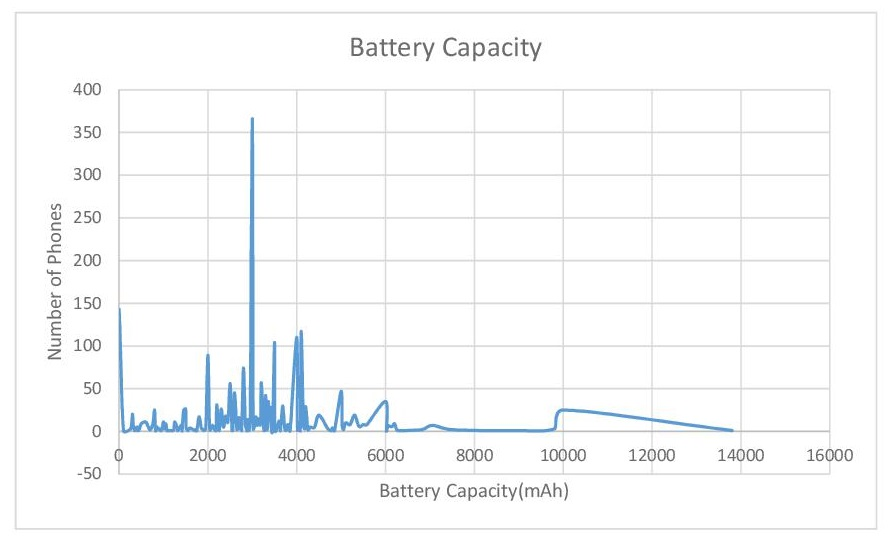
\includegraphics[width=15.00cm]{3.jpg}\\
  \caption{Line Chart of Battery Capacity. The Capacity focuses on 3000, 4000, and 4100 mAh.}\label{fig3}
\end{figure}

\begin{figure}
  \centering
  % Requires \usepackage{graphicx}
  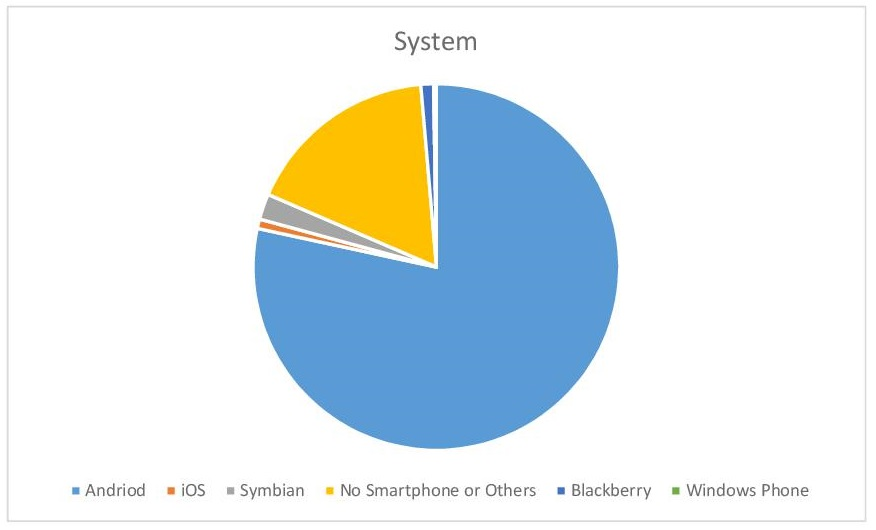
\includegraphics[width=15.00cm]{4.jpg}\\
  \caption{Pie Chart of System. The Android system takes a major proportion.}\label{fig4}
\end{figure}


\begin{table}
  \centering
  \begin{tabular}{|l|l|l|l|l|l|}
\hline
\multicolumn{1}{|c|}{}                                                         & 1  & 2  & 3  & 4  & 5  \\ \hline
\begin{tabular}[c]{@{}l@{}}Lower than\\   3000\end{tabular}                    & 93 & 67 & 92 & 88 & 14 \\ \hline
3000                                                                           & 59 & 40 & 66 & 60 & 8  \\ \hline
\begin{tabular}[c]{@{}l@{}}More than\\   3000  but less than 4000\end{tabular} & 80 & 57 & 85 & 79 & 16 \\ \hline
\begin{tabular}[c]{@{}l@{}}4000mAh to\\   4100\end{tabular}                    & 24 & 19 & 53 & 60 & 42 \\ \hline
\begin{tabular}[c]{@{}l@{}}More than\\   4100\end{tabular}                     & 73 & 39 & 64 & 37 & 9  \\ \hline
\end{tabular}
  \caption{ Statistics from Battery Capacity to Click Rate Category. The upper-middle Battery Capacity reveals a better sales. }\label{Basic Statistics}
\end{table}


 Figure 3 demonstrate, for instance: most of the phones possess 3000 mAh, 4000 mAh, or 4100 mAh battery. The phones with Android systems lead the ranking of systems, while Apple system is the second one. For the phones which achieve higher click rate category, they are more likely to have the upper-middle battery capacity.

\subsection{Weight Determination Technique}

\textbf{In order to choose by diverse factors and judge the sales of certain types of phones, we create a new Weight Determination Technique, which imitates the Analytic Hierarchy Process (AHP), to achieve the goal which is to qualitatively determine the weight of each option in complicated and uncertain problems. }We define the properties of the phones, which are display resolution, recording definition, RAM, ROM, CPU core, highest camera resolution, and price, obtained from the Principal Component Analysis, as the scheme layer, while defining the click rate and the convert rate as the target layer, to build up the weight determining model with one mere layer but several groups, which is shown in table \ref{fig5}.

\begin{figure}
  \centering
  % Requires \usepackage{graphicx}
  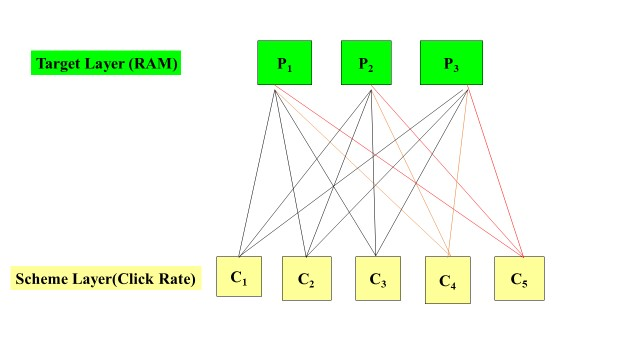
\includegraphics[width=15.00cm]{5.jpg}\\
  \caption{Structure diagram. We use only two layers but with several groups.}\label{fig5}
\end{figure}

We divide RAM into three groups, less than 1 GB, no less than 1 GB but less than 4 GB, and more than 4 GB, of which are groups 1, 2, and 3 respectively. We divide ROM into three groups, less than 8 GB, no less than 8 GB but less than 64 GB, and more than 64 GB, of which are groups 1, 2, and 3 respectively. We also divide display resolution, recording definition, highest camera resolution, and price into several categories, of which the standard is the same as what we do in the Information Entropy part. Figure 5 shows the diagram from RAM to click rate.  [14]

First, we define the amounts of phones that possess certain properties under certain types of sales conditions, which refers to the amount of a certain target choice under a certain scheme layer condition, as w. In accordance with the target choice, we obtain a weight vector $\left( \begin{array} { l l l } { w _ { 1 } } & { \dots } & { w _ { n } } \end{array} \right)$(n stands for the number of choices of target layer). We compute the ratio between the number, $w _ { i } ( 1 \leq i \leq n )$, of each scheme layer choice under a common target layer choice and regard it as the weight of paired comparison matrix. As they are consistent matrixes, we do not need to apply consistency tests to the matrixes, for they are automatically consistent, which means that the eigenvalues are all identical. With the help of the formula of the eigenvalue and eigenvectors shown in formula \ref{for20},

\begin{equation}\label{for20}
A \omega = \lambda \omega
\end{equation}

we can obtain the eigenvectors, $\omega$. Composing the eigenvalues of each scheme layer, we obtain the eigenvector matrixes as well as weight vector matrixes from the target layer to the scheme layer.

Then we repeat the process from each scheme layer, which is the sales condition, to each target layer, which is the properties of the phones, to achieve the goal that for each scheme the sum of the weight vector is 1 to transversely compare which option is more welcomed under the same sales condition. Comparing the weight of each scheme to one single target vertically, we obtain which kinds of phones are more welcomed under the same standard.

Finally, we draw the statistical chart with each weight vector, such as stacked column charts, to clearly express the interference of the properties of the phones to the result. The charts are shown in the appendix, one of which is shown in figure \ref{fig6}.

\begin{figure}
  \centering
  % Requires \usepackage{graphicx}
  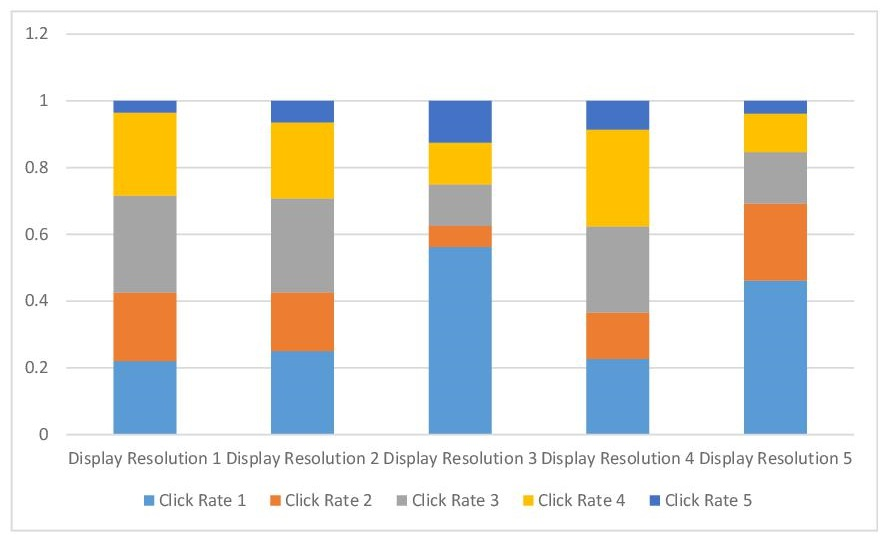
\includegraphics[width=15.00cm]{6.jpg}\\
  \caption{Result analysis. The middle Display Resolution experiences both a better sale and a worse sale.}\label{fig6}
\end{figure}


We can clearly see that phones with middle display resolution tend to attract more customer to click in and purchase. Phones with lower and higher recording definition are more welcomed, while phones with medium counterpart are less intriguing. Phones with lower RAM, ROM, and CPU involve in more click rate, whereas phones with higher equivalents involve in more convert rate. For both highest camera resolution and price, the medium ones are both attractive.

\textbf{It is obvious that a qualitative analysis is not ample for the issue, which indicates we need to do further analysis.}

\subsection{Logistic Regression}

Before Logistic Regression, we consider a third model to be Linear Regression. The third modeling method we use is Linear Regression. We can regard the properties of phones as independent variables, and the sales as dependent variables. Based on the samples, each data can be viewed as a mapping from the independent variables, which are the properties, to the dependent variables, which are sales. As each information is expressed numerical, we can find the function from the independent variables to the dependent variables through linear regression from the data. [15]

Let $x _ { 1 }$ to $x _ { 7 }$ respectively denote display resolution, recording definition, RAM, ROM, CPU core, highest camera resolution, and price. Let $y _ { 1 }$ denotes click rate and $y _ { 2 }$ denote convert rate. The value of the independent variables and dependent variables is the numbers of each option. We utilize regression formula \ref{for21}.

\begin{equation}\label{for21}
y _ { n } = \beta _ { 0 } + \beta _ { 1 } x _ { 1 } + \beta _ { 2 } x _ { 2 } + \beta _ { 3 } x _ { 3 } + \beta _ { 4 } x _ { 4 } + \beta _ { 5 } x _ { 5 } + \beta _ { 6 } x _ { 6 } ( n \in \{ 1,2 \} )
\end{equation}

Let $X$ denotes the independent variables matrix;$Y _ { n } \left( n \in \left\{ n \in N ^ { * } | n \leq 2 \right\} \right)$ denote dependent variables matrixes; $\beta$ denotes coefficient matrixes. We apply Least Square Regression Method to the issue, of which the formula is shown in formula \ref{for22}.

\begin{equation}\label{for22}
\beta ^ { \prime } = \left( X ^ { T } X \right) ^ { - 1 } X ^ { T } Y = \left( \sum x _ { i } x _ { i } ^ { T } \right) ^ { - 1 } \left( \sum x _ { i } y _ { i } \right) \left( i \in \left\{ i \in N ^ { * } | i \leq n \right\} \right)
\end{equation}

The formula is set to solve out the value of the coefficient matrixes of point estimation. With MATLAB giving solution, we obtain the coefficient matrixes which are presented in table \ref{Linear Regression Coefficients}.

\begin{table}
  \centering
  \begin{tabular}{|l|l|l|}
\hline
\multicolumn{1}{|c|}{}                        & Click Rate & Convert Rate \\ \hline
\begin{tabular}[c]{@{}l@{}}$\beta_0$ \end{tabular} & 0.015683   & 0.016454     \\ \hline
\begin{tabular}[c]{@{}l@{}}$\beta_1$\end{tabular} & 8.16E-10   & 6.63E-10     \\ \hline
\begin{tabular}[c]{@{}l@{}}$\beta_2$\end{tabular} & 2.12E-06   & 1.94E-06     \\ \hline
\begin{tabular}[c]{@{}l@{}}$\beta_3$\end{tabular} & -0.0004    & -0.0004      \\ \hline
\begin{tabular}[c]{@{}l@{}}$\beta_4$\end{tabular} & 9.24E-06   & 9.30E-06     \\ \hline
\begin{tabular}[c]{@{}l@{}}$\beta_5$\end{tabular} & 3.86E-05   & -1.99E-05    \\ \hline
\begin{tabular}[c]{@{}l@{}}$\beta_6$\end{tabular} & 2.55E-05   & 1.99E-05     \\ \hline
\begin{tabular}[c]{@{}l@{}}$\beta_7$\end{tabular} & -1.04E-05  & -9.99E-06    \\ \hline
\end{tabular}
  \caption{Linear Regression Coefficients}\label{Linear Regression Coefficients}
\end{table}

Point estimation possesses a drawback that it cannot express the accuracy of the data obtained. Thus we utilize interval estimation to reuse the Least Square Regression Method, the formula as in formula \ref{for23}.

\begin{equation}\label{for23}
P \left\{ \hat { \theta } _ { 1 } < \theta < \widehat { \theta } _ { 2 } \right\} = 1 - \alpha
\end{equation}

$\theta$ denotes the parameters to be estimated of the ensemble; $P$ denotes probability; $\hat { \theta } _ { 1 }$ denotes Confidence upper limit; $\hat { \theta } _ { 2 }$ denotes Confidence lower limit; $\alpha$ denotes reliability which satisfies $0 < \alpha < 1$. In this way, we obtain formula \ref{for24}.

\begin{equation}\label{for24}
P \left\{ \hat { \beta } _ { n 1 } < \beta < \hat { \beta } _ { n 2 } \right\} = 1 - \alpha \left( n \in \left\{ n \in N ^ { * } | n \leq 2 \right\} \right)
\end{equation}

With the MATLAB program, we set $\alpha$ as 0.95, under which the regression coefficient bound is shown in table \ref{Linear Regression Coefficient Bound}.


\begin{table}
  \centering
  \begin{tabular}{|l|l|l|l|l|}
\hline
\multicolumn{1}{|c|}{} & \begin{tabular}[c]{@{}l@{}}Click Rate Lower\\   Bound\end{tabular} & \begin{tabular}[c]{@{}l@{}}Convert Rate\\   Lower Bound\end{tabular} & \begin{tabular}[c]{@{}l@{}}Click Rate Upper\\   Bound\end{tabular} & \begin{tabular}[c]{@{}l@{}}Convert Rate\\   Upper Bound\end{tabular} \\ \hline
$\beta_0$                    & 0.01178                                                            & 0.012596                                                             & 0.019587                                                           & 0.020311                                                             \\ \hline
$\beta_1$                    & -4.83E-10                                                          & -6.20E-10                                                            & 2.11E-09                                                           & 1.95E-09                                                             \\ \hline
$\beta_2$                  & -1.79E-06                                                          & -1.92E-06                                                            & 6.03E-06                                                           & 5.81E-06                                                             \\ \hline
$\beta_3$                    & -0.00125                                                           & -0.00123                                                             & 0.000441                                                           & 0.000437                                                             \\ \hline
$\beta_4$                    & -3.04E-05                                                          & -2.99E-05                                                            & 4.89E-05                                                           & 4.85E-05                                                             \\ \hline
$\beta_5$                    & -0.00047                                                           & -0.00057                                                             & 0.00055                                                            & 0.000438                                                             \\ \hline
$\beta_6$                   & -0.00016                                                           & -0.00017                                                             & 0.000213                                                           & 0.000205                                                             \\ \hline
$\beta_7$                    & -1.78E-05                                                          & -1.73E-05                                                            & -3.02E-06                                                          & -2.68E-06                                                            \\ \hline
\end{tabular}
  \caption{Linear Regression Coefficient Bound}\label{Linear Regression Coefficient Bound}
\end{table}

Residual graphs are in the appendix, one of which is shown in figure \ref{fig7}. When examining correlation coefficients, we find the correlation coefficients are as presented in table \ref{Linear Regression Correlation Coefficients}.

\begin{figure}
  \centering
  % Requires \usepackage{graphicx}
  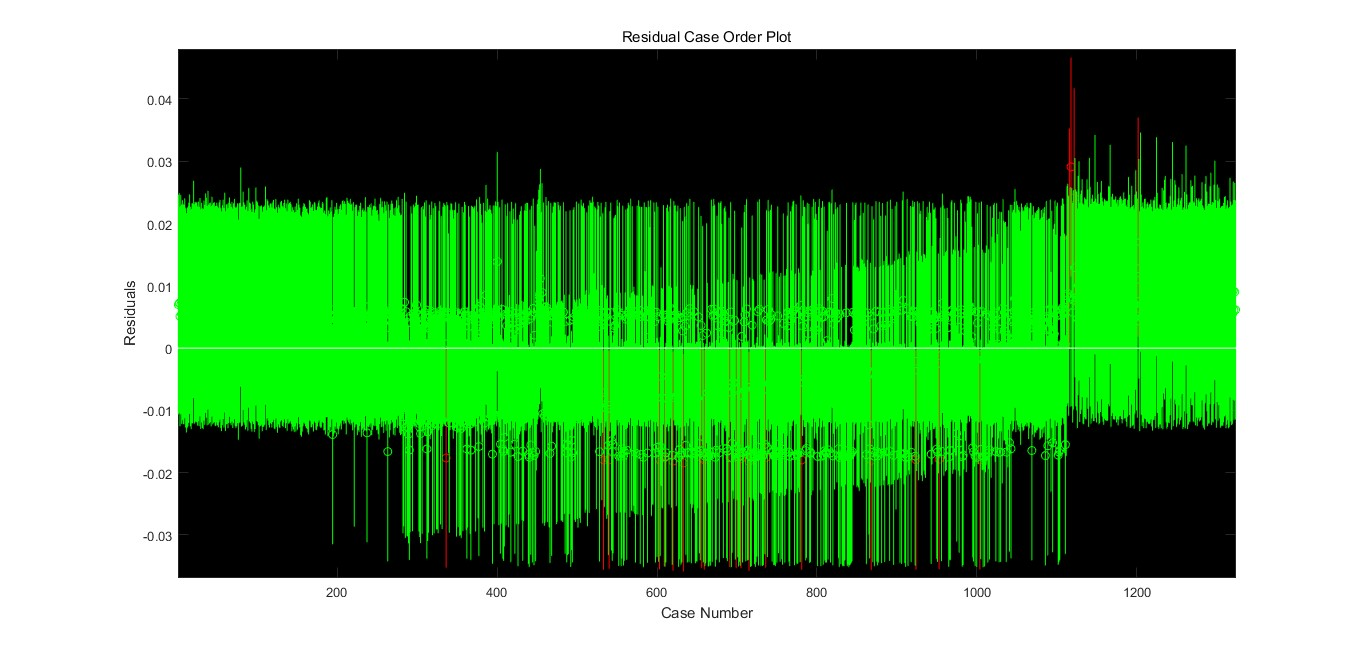
\includegraphics[width=15.00cm]{7.jpg}\\
  \caption{Residual Case Order Plot of Linear Regression}\label{fig7}
\end{figure}

\begin{table}
  \centering
  \begin{tabular}{|l|l|}
\hline
\multicolumn{1}{|c|}{Click Rate} & Convert Rate \\ \hline
0.011098                         & 0.01021      \\ \hline
\end{tabular}
  \caption{Linear Regression Correlation Coefficients, which is not high enough for further analysis. }\label{Linear Regression Correlation Coefficients}
\end{table}

Moreover, we find the Linear Regression model flaws in failing to consider the lower and upper bound of the data. For instance, the click rate and convert rate must be lower than 1 but no less than 0, which means is locates in the [0, 1) interval, while Linear Regression cannot set such a bound. \textbf{Thus, with the formula listed above, we further use General Linear Model to solve the problem, specifically Logistic regression, to add the lower and upper bond of the regression model. }We add a transfer function from the output of the linear model to the final output and redo the regression. The transfer function is set as Sigmond Function, of which the formula is as following formula \ref{for25}.

\begin{equation}\label{for25}
y ( x ) = \frac { 1 } { 1 + e ^ { - x } }
\end{equation}

The regression coefficients are shown in table \ref{Logistic Regression Coefficient}.

\begin{table}
  \centering
  \begin{tabular}{|l|l|l|}
\hline
\multicolumn{1}{|c|}{} & Click Rate & Convert Rate \\ \hline
$\beta_0$                       & -4.13968   & -4.09207     \\ \hline
$\beta_1$                       & 5.75E-08   & 4.73E-08     \\ \hline
$\beta_2$                       & 0.000124   & 0.000113     \\ \hline
$\beta_3$                      & -0.02237   & -0.0221      \\ \hline
$\beta_4$                       & 0.000887   & 0.000862     \\ \hline
$\beta_5$              & 0.003291   & -0.00332     \\ \hline
$\beta_6$     & 0.001981   & 0.001606     \\ \hline
 $\beta_7$& -0.00084   & -0.00079     \\ \hline
\end{tabular}
  \caption{Logistic Regression Coefficients}\label{Logistic Regression Coefficient}
\end{table}


\textbf{In light of the low correlation coefficients in Linear Regression, which is insufficient to reveal the features of each variable precisely, we consider revising the methods to achieve a better performance.}

\subsection{KNN Algorithm}

In accordance with the given data, we try to randomly sample two-thirds of the data as learning samples and one-third of the data as the test data to highly merge the vast amount of the data and find the shared features and characteristics of each sample to obtain the common properties of the phones under similar sales condition to determine the relationship. [16]

We utilize Mahalanobis distance distinction to operate these data, which is processed after principal component analysis and features eradicating the dimension of each independent variables. The formula is shown as formula \ref{for26}.

\begin{equation}\label{for26}
d ( x , y ) = \sqrt { ( x - y ) \Sigma ^ { - 1 } ( x - y ) ^ { T } }
\end{equation}

Among the formula, $x$ and $y$ denote two row vectors; $\Sigma$ denotes the covariance matrix; $d ( x ,y )$ denotes the obtained Mahalanobis distance of the data.

For the click rate, we correctly categorized 51 samples out of 444, \textbf{achieving an accuracy of 11\%}; for the convert rate, we correctly categorized 72 samples out of 444, \textbf{achieving an accuracy of 16\%, which is too low for further application}. Thus, we made an optimization in 5.2.
\section{Optimization}
\subsection{Principal Component Regression}

\textbf{Principal Component Regression suits explicitly for the problems that have a vast amount of independent data types, not all of which are tightly connected to the dependent data, which means some of the data are loosely related to the data. In view of considering that our problem has 26 independent variables, the method is highly compatible with our research. First we carry out Linear Regression with PCA, then we carry out Logistic Regression with PCA.}

We can still do as part 3.4, regarding the sales condition as dependent variables and the properties of phones as independent variables. We try to reduce the dimensionality, reducing the vast amount of the original data and variables into fewer data and variables, while the new variables can retain the information in the original data by and large. [17]

We utilize the 26 original variables mentioned in 3.4 as the original data. We still use X to denote independent variables matrixes and $Y _ { n } \left( n \in \left\{ n \in N ^ { * } | n \leq 2 \right\} \right)$ to denote the two dependent variables. The original variables are $x _ { p } \left( p \in \left\{ p \in N ^ { * } | p \leq l \right\} \right)$; the new variables are $z _ { q } \left( q \in \left\{ q \in N ^ { * } | q \leq p \right\} \right)$. We use m to denote the number of samples and use l to denote the number of variables in each sample.

Applying Least squares regression, point estimation and interval estimation method which has previously been mentioned, we obtain the principal coefficient matrix $��'$ as shown in table \ref{Coefficient Matrix of principal component} with formula \ref{for27}.

\begin{equation}\label{for27}
y _ { n } ^ { * } = \beta _ { 1 } ^ { \prime } z _ { 1 } + \beta _ { 2 } ^ { \prime } z _ { 2 } + \beta _ { 3 } ^ { \prime } z _ { 3 } + \cdots + \beta _ { 14 } ^ { \prime } z _ { 14 } \left( n \in \left\{ n \in N ^ { * } | n \leq 2 \right\} \right)
\end{equation}

\begin{table}
  \centering
  \begin{tabular}{|l|l|l|l|l|l|}
\hline
\multicolumn{1}{|c|}{Click rate} & Convert rate & \multicolumn{2}{l|}{Click rate bond} & \multicolumn{2}{l|}{Convert rate bond} \\ \hline
0.0060599                        & 0.0056618    & 0.003038          & 0.009082         & 0.002802           & 0.008522          \\ \hline
-5.91E-05                        & -4.68E-05    & -0.00016          & 4.42E-05         & -0.00014           & 5.10E-05          \\ \hline
0.0022433                        & 2.28E-03     & 0.002098          & 0.002389         & 0.002139           & 0.002414          \\ \hline
0.0005191                        & 0.0004617    & 0.000334          & 0.000705         & 0.000286           & 0.000637          \\ \hline
-0.001295                        & -0.001239    & -0.00149          & -0.0011          & -0.00143           & -0.00105          \\ \hline
0.0023177                        & 0.0024434    & 0.002098          & 0.002538         & 0.002235           & 0.002652          \\ \hline
-0.00197                         & -0.001954    & -0.0022           & -0.00174         & -0.00217           & -0.00174          \\ \hline
-0.002325                        & -0.002318    & -0.00256          & -0.00209         & -0.00254           & -0.00209          \\ \hline
-0.001023                        & -0.001066    & -0.00126          & -0.00078         & -0.00129           & -0.00084          \\ \hline
0.0014761                        & 0.0014155    & 0.001225          & 0.001727         & 0.001178           & 0.001653          \\ \hline
0.0035007                        & 0.0034757    & 0.003248          & 0.003754         & 0.003236           & 0.003715          \\ \hline
-0.000469                        & -0.000463    & -0.00073          & -0.00021         & -0.00071           & -0.00022          \\ \hline
0.0026733                        & 0.0026214    & 0.002411          & 0.002936         & 0.002373           & 0.00287           \\ \hline
0.0007999                        & 0.000746     & 0.000525          & 0.001075         & 0.000486           & 0.001006          \\ \hline
-0.003063                        & -0.00304     & -0.00334          & -0.00278         & -0.0033            & -0.00278          \\ \hline
\end{tabular}
  \caption{Coefficient Matrix of principal component}\label{Coefficient Matrix of principal component}
\end{table}

The correlation coefficients of this method are shown in table \ref{PCA Correlation Coefficients}, which are satisfactory for further calculation.

\begin{table}
  \centering
  \begin{tabular}{|l|l|}
\hline
\multicolumn{1}{|c|}{Click Rate} & Convert Rate \\ \hline
0.805032                         & 0.826614      \\ \hline
\end{tabular}
  \caption{Principal Component Regression Correlation Coefficients, which shows that the model is accurate. }\label{PCA Correlation Coefficients}
\end{table}

Ultimately, we conduct the inverse standardization process and obtain the equation interpreted in the original data, which is formula \ref{for28}, and the final coefficient matrix, as shown in table \ref{Corfficient Matrix of PCR}.

\begin{table}
  \centering
  \begin{tabular}{|l|l|l|l|l|l|}
\hline
\multicolumn{1}{|c|}{Click rate} & Convert rate & \multicolumn{2}{l|}{Click rate Bound} & \multicolumn{2}{l|}{Convert Rate Bound} \\ \hline
0.0060599                        & 0.0056618    & 0.0030378         & 0.009082          & 0.0028019          & 0.0085217          \\ \hline
-0.000416                        & -0.000432    & -0.000728         & -0.000104         & -0.000727          & -0.000136          \\ \hline
-0.000741                        & -7.23E-04    & -0.00085          & -6.32E-04         & -0.000827          & -6.20E-04          \\ \hline
8.15E-04                         & 8.05E-04     & 0.0004825         & 0.0011472         & 0.0004903          & 0.0011194          \\ \hline
6.45E-04                         & 6.25E-04     & 0.0006069         & 0.0006826         & 0.0005892          & 0.0006609          \\ \hline
5.33E-05                         & -2.88E-05    & -0.000243         & 0.0003497         & -0.000309          & 0.0002516          \\ \hline
6.66E-06                         & 6.73E-05     & -0.000168         & 0.0001809         & -9.77E-05          & 0.0002322          \\ \hline
-4.21E-05                        & -4.43E-05    & -5.70E-05         & -2.71E-05         & -5.85E-05          & -3.02E-05          \\ \hline
0.0003321                        & 0.0003663    & 0.0001684         & 0.0004958         & 0.0002114          & 0.0005212          \\ \hline
-1.58E-04                        & -1.42E-04    & -2.08E-04         & -1.09E-04         & -1.88E-04          & -9.45E-05          \\ \hline
-1.33E-04                        & -1.17E-04    & -0.000163         & -1.04E-04         & -0.000144          & -8.83E-05          \\ \hline
8.80E-05                         & 8.91E-05     & 0.0001985         & -2.26E-05         & 0.0001938          & -1.54E-05          \\ \hline
6.22E-06                         & -2.70E-05    & 3.34E-05          & -2.10E-05         & -1.08E-06          & -5.25E-05          \\ \hline
-1.02E-04                        & -5.88E-05    & -0.000185         & -1.80E-05         & -0.000138          & 2.04E-05           \\ \hline
1.03E-05                         & -7.27E-07    & -5.68E-05         & 7.73E-05          & -6.41E-05          & 6.28E-05           \\ \hline
-7.90E-05                        & -6.13E-05    & -0.000183         & 2.53E-05          & -0.00016           & 3.74E-05           \\ \hline
-0.00123                         & -0.001159    & -0.001532         & -0.000929         & -0.001444          & -0.000873          \\ \hline
-3.70E-04                        & -3.43E-04    & -0.000322         & -0.000419         & -0.000297          & -0.000388          \\ \hline
0.00049                          & 4.09E-04     & 0.0002795         & 0.0007006         & 0.0002093          & 0.0006079          \\ \hline
0.0017751                        & 0.0018274    & 0.0018016         & 0.0017487         & 0.0018521          & 0.0018021          \\ \hline
2.02E-04                         & 2.12E-04     & 2.30E-04          & 1.74E-04          & 2.39E-04           & 1.86E-04           \\ \hline
3.89E-04                         & 4.09E-04     & 2.98E-04          & 4.80E-04          & 3.21E-04           & 4.94E-04           \\ \hline
6.14E-04                         & 6.37E-04     & 5.44E-04          & 6.83E-04          & 5.69E-04           & 7.01E-04           \\ \hline
0.0006015                        & 0.0006246    & 0.0005317         & 0.0006714         & 0.0005567          & 0.0006889          \\ \hline
0.0067859                        & 0.0067646    & 0.0067075         & 0.0068643         & 0.0066899          & 0.0068383          \\ \hline
0.0006558                        & 0.0006962    & 0.000579          & 0.0007326         & 0.0006229          & 0.0007682          \\ \hline
0.0002644                        & 0.0002347    & -0.000138         & 0.0006663         & -0.000145          & 0.0006153          \\ \hline
\end{tabular}
  \caption{Coefficient Matrix of original variables of Principal Component Regression}\label{Corfficient Matrix of PCR}
\end{table}


\begin{equation}\label{for28}
y _ { n } = \beta _ { 0 } + \beta _ { 1 } x _ { 1 } + \beta _ { 2 } x _ { 2 } + \beta _ { 3 } x _ { 3 } + \cdots + \beta _ { 26 } x _ { 26 } ( n \in \{ 1,2 \} )
\end{equation}

As what we have done in part 4.3, we do the Logistic Regression and find the following coefficients in table \ref{Final Coefficient Matrix}.

\begin{table}
  \centering
  \begin{tabular}{l|l|l|l|}
\hline
\multicolumn{1}{|c|}{Click rate of Principal} & \begin{tabular}[c]{@{}l@{}}Convert rate of\\   Principal\end{tabular} & \begin{tabular}[c]{@{}l@{}}Click Rate of\\   Original\end{tabular} & Convert Rate of Original \\ \hline
\multicolumn{1}{|l|}{-5.15504}                & 0.0056618                                                             & -5.17865                                                           & -5.17865                 \\ \hline
\multicolumn{1}{|l|}{-0.01171}                & -0.000432                                                             & -0.01084                                                           & -0.03205                 \\ \hline
\multicolumn{1}{|l|}{0.144798}                & -7.23E-04                                                             & 0.144825                                                           & -0.06438                 \\ \hline
\multicolumn{1}{|l|}{0.040233}                & 8.05E-04                                                              & 0.036409                                                           & 0.056077                 \\ \hline
\multicolumn{1}{|l|}{-0.12243}                & 6.25E-04                                                              & -0.11859                                                           & 0.051036                 \\ \hline
\multicolumn{1}{|l|}{0.205632}                & -2.88E-05                                                             & 0.211749                                                           & -0.00208                 \\ \hline
\multicolumn{1}{|l|}{-0.15896}                & 6.73E-05                                                              & -0.15702                                                           & 0.00477                  \\ \hline
\multicolumn{1}{|l|}{-0.18697}                & -4.43E-05                                                             & -0.18577                                                           & -0.00774                 \\ \hline
\multicolumn{1}{|l|}{-0.1002}                 & 0.0003663                                                             & -0.10133                                                           & 0.027024                 \\ \hline
\multicolumn{1}{|l|}{0.121211}                & -1.42E-04                                                             & 0.117731                                                           & -0.01077                 \\ \hline
\multicolumn{1}{|l|}{0.29027}                 & -1.17E-04                                                             & 0.286483                                                           & -0.00786                 \\ \hline
\multicolumn{1}{|l|}{-0.04298}                & 8.91E-05                                                              & -0.04205                                                           & 0.011503                 \\ \hline
\multicolumn{1}{|l|}{0.219448}                & -2.70E-05                                                             & 0.214352                                                           & -0.00041                 \\ \hline
\multicolumn{1}{|l|}{0.073279}                & -5.88E-05                                                             & 0.070026                                                           & -0.00416                 \\ \hline
\multicolumn{1}{|l|}{-0.25463}                & -7.27E-07                                                             & -0.25096                                                           & -0.00172                 \\ \hline
                                              & -6.13E-05                                                             &                                                                    & -0.00201                 \\ \cline{2-2} \cline{4-4}
                                              & -0.001159                                                             &                                                                    & -0.08629                 \\ \cline{2-2} \cline{4-4}
                                              & -3.43E-04                                                             &                                                                    & -0.03116                 \\ \cline{2-2} \cline{4-4}
                                              & 4.09E-04                                                              &                                                                    & 0.03289                  \\ \cline{2-2} \cline{4-4}
                                              & 0.0018274                                                             &                                                                    & 0.163717                 \\ \cline{2-2} \cline{4-4}
                                              & 2.12E-04                                                              &                                                                    & 0.019238                 \\ \cline{2-2} \cline{4-4}
                                              & 4.09E-04                                                              &                                                                    & 0.010522                 \\ \cline{2-2} \cline{4-4}
                                              & 6.37E-04                                                              &                                                                    & 0.02587                  \\ \cline{2-2} \cline{4-4}
                                              & 0.0006246                                                             &                                                                    & 0.024865                 \\ \cline{2-2} \cline{4-4}
                                              & 0.0067646                                                             &                                                                    & 0.556614                 \\ \cline{2-2} \cline{4-4}
                                              & 0.0006962                                                             &                                                                    & 0.044207                 \\ \cline{2-2} \cline{4-4}
                                              & 0.0002347                                                             &                                                                    & 0.019128                 \\ \cline{2-2} \cline{4-4}
\end{tabular}
  \caption{Final Coefficient Matrix of original variables}\label{Final Coefficient Matrix}
\end{table}



\textbf{Principal Component Regression features a significant weakness that it cannot portray the discrete variables perfectly, which means we need further optimization.}

\subsection{Bayes Distinction}

Bayes Distinction ideally satisfies the requirements of such issue that each individual of the ensemble exists at different frequencies, which indicates that we need to take into consideration that the different possibilities that each individual exists. \textbf{As for our research, each phone is obviously impossible to appear at identical frequencies, so we apply Bayes Distinction to our study.}

In the distance distinction method above, it does not take into account the frequency of each sample in the whole and does not take into account the loss caused by the wrong distinction. The Bayes distinction method modifies on the basis of distance distinction, and the formula is defined as in formula \ref{for29}. [18]

\begin{equation}\label{for29}
P \left( B _ { i } | A \right) = \frac { P ( A | B _ { i } ) P \left( B _ { i } \right) } { \sum P ( A | B _ { j } ) P \left( B _ { i } \right) }
\end{equation}

Among which $P \left( B _ { i } | A \right)$ represents a posteriori probability; $P ( A | B _ { i } )$ represents a prior probability; $P \left( B _ { i } \right)$ represents the frequency at which the sample appears; �� represents the total covariance matrixes. The distinction rule is that the posterior probability is the highest and the average wrong distinction loss is the lowest, which brings out the rule is as follows: If the condition meets the following formula \ref{for30}:

\begin{equation}\label{for30}
P \left( G _ { l } | x _ { 0 } \right) = \frac { p _ { 1 } f _ { l } \left( x _ { 0 } \right) } { \Sigma p _ { j } f _ { j } \left( x _ { 0 } \right) }=\max _ {  1 \leq i \leq k  } \frac { p _ { i } f _ { i } \left( x _ { 0 } \right) } { \Sigma p _ { j } f _ { j } \left( x _ { 0 } \right) }
\end{equation}

Then we categorize $x _ { 0 }$ into $G _ { l }$, among which $G _ { i }$ is the ensemble, $f ( x )$ is the probability density function of $G _ { i _ { 2 } }, p _ { i }$ is prior probability of $G _ { i }$ , which is the probability that it belongs a certain category when sample  $x _ { 0 }$ occurs, and k is the number of $G _ { i }$ . The solution formula for distinction analysis is as the following formulas \ref{for31}-\ref{for32}.

\begin{equation}\label{for31}
E C M = \sum _ { i = 1 } ^ { k } p _ { i } \sum _ { j \neq i } C ( \frac{j}{i} ) P ( \frac{j}{i} )
\end{equation}

\begin{equation}\label{for32}
p ( \frac{j}{i} ) = P \left( X \in D _ { j } / G _ { i } \right) = \int _ { D _ { j } } f _ { i } ( x ) d x \quad i \neq j
\end{equation}



In this case, $P ( \frac{j}{i} )$ represents the conditional probability of wrongly categorizing the sample of $G _ { i }$ to the ensemble $G _ { j }( \frac{j}{i} )$ is the loss caused by this categorization. $D _ { k}$ is a division of a set of distinction samples. $ECM$ is the average wrong distinction loss. The solution to a Bayes distinction analysis is to make the smallest set of solutions.

\begin{figure}
  \centering
  % Requires \usepackage{graphicx}
  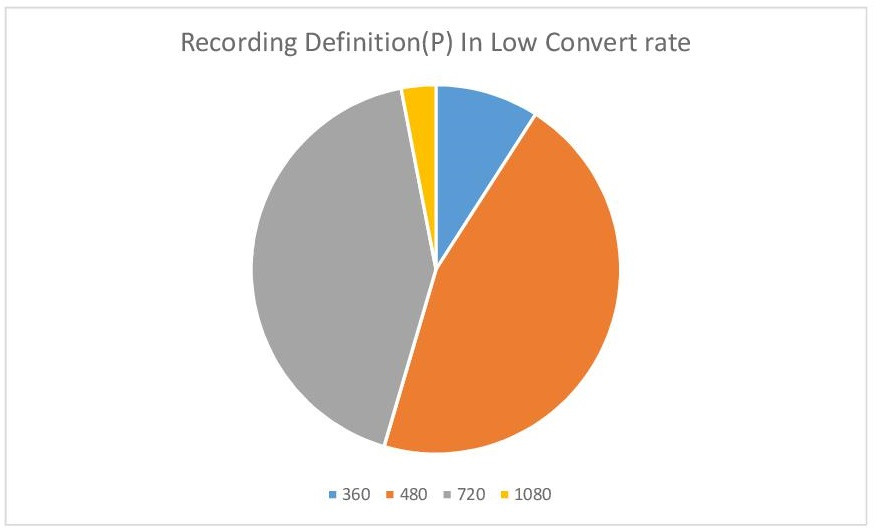
\includegraphics[width=15.00cm]{8.jpg}\\
  \caption{Bayes Result of Recording Definition in Low Convert Rate. Lower Recording Definition has a relatively lower Convert Rate.}\label{fig8}
\end{figure}


Using the MATLAB program, we still randomly sample $\frac{2}{3}$ of the ensemble as a learning sample and $\frac{1}{3}$ as a test set to carry out Bayes distinction solution. We utilize the data after principal component analysis to study the condition of the distinction.
The result is shown in the appendix, part of which is as following figure \ref{fig8}-\ref{fig9} and table \ref{Bayes}. For instance, the number ``p91" shows that there are 91 samples with 2G RAM are judged as click rate category 1.

\begin{table}
  \centering
  \begin{tabular}{|l|l|l|l|l|}
\hline
\multicolumn{1}{|c|}{} & Category 1 & Category 2 & Category 3 & Category 4 \\ \hline
0.125                  & 2          & 0          & 0          & 0          \\ \hline
0.5                    & 7          & 0          & 0          & 1          \\ \hline
1                      & 49         & 0          & 1          & 7          \\ \hline
1.5                    & 1          & 0          & 0          & 0          \\ \hline
2                      & 91         & 0          & 15         & 25         \\ \hline
3                      & 41         & 1          & 64         & 19         \\ \hline
4                      & 1          & 13         & 68         & 2          \\ \hline
6                      & 0          & 11         & 22         & 0          \\ \hline
8                      & 0          & 0          & 1          & 0          \\ \hline
\end{tabular}
  \caption{RAM result in click rate. Both better sales and worse sales focus on higher RAM. }\label{Bayes}
\end{table}


For the click rate, we correctly categorized 89 samples out of 444, achieving an accuracy of 20\%; for the convert rate, we correctly categorized 176 samples out of 444, achieving an accuracy of 40\%, which is relatively higher than the accuracy obtained from KNN algorithm.

\begin{figure}
  \centering
  % Requires \usepackage{graphicx}
  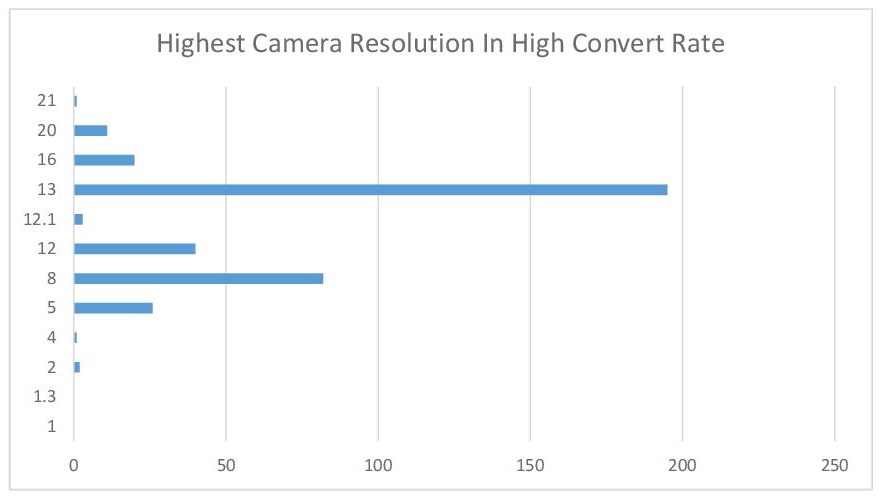
\includegraphics[width=15.00cm]{9.jpg}\\
  \caption{Bayes Result of Highest Camera Resolution in High Convert Rate. Phones with Higher Camera Resolution demonstrates better sales.}\label{fig9}
\end{figure}

From the results given, we can clearly figure out the trend that the higher the mobile configuration is, the high click rate and convert rate the sample has. To be specific, phones with higher display resolution, higher recording definition, higher camera resolution, more CPU cores, larger RAM, and more spacious ROM are apt to reveal more satisfactory sales condition. The phones that display weaker sales performance tend to possess lower counterparts of the features listed above.

\textbf{Bayes Distinction has a drawback that the results it gives out are discrete, while the click rate and convert rate ought to be continuous, which means we need further optimization.}

\subsection{BP Neural Network Fitting}

BP Neural Network is a kind of multilayer feed-forward network, \textbf{which highly fits for the problem that there are data with a certain scale, the relationship between which is not too complicated to identify. }When it comes to our target, we have a middle-sized database, while the process we want is fitting, which is not too intricate, which shows that the model can be applied to our goal.

We utilize BP neural network fitting as another method to promote the accuracy of the regression. BP neural network works to encode itself with its high-dimensional features and to carry out dimension reduction processing towards high-dimensional data. It is marked by a feature extraction model with unsupervised learning, which can also combine a few basic features to obtain higher-layer abstract features. [19]

We utilize Tangent Sigmoid function as the transfer function; we use Levenberg Marquardt algorithm (trainlm) as the training algorithm; we use the Gradient descent with momentum weight and bias learning function (learngdm) as the learning algorithm; we use the mean square error (MSE) method as the learning function. The structure of the network and the performance plot are shown in figure \ref{fig10} and \ref{fig11}.

\begin{figure}
  \centering
  % Requires \usepackage{graphicx}
  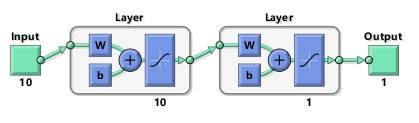
\includegraphics[width=15.00cm]{10.jpg}\\
  \caption{BP Neural Network Structure. The layer number, which is 10, does not consumes too much time while the result is satisfactory.}\label{fig10}
\end{figure}


\begin{figure}
  \centering
  % Requires \usepackage{graphicx}
  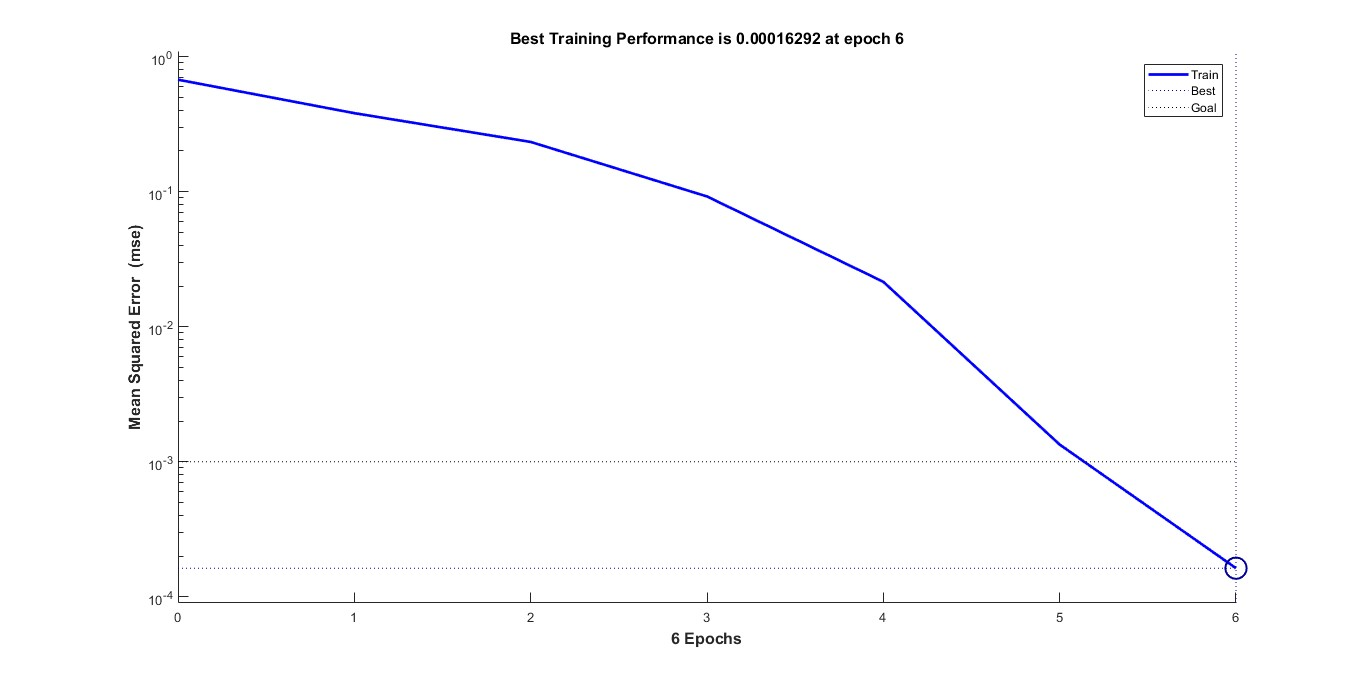
\includegraphics[width=15.00cm]{11.jpg}\\
  \caption{The performance plot of BP Neural Network. The training performance is enhancing rapidly.}\label{fig11}
\end{figure}


We utilize the properties after the Information Entropy analysis to conduct the process. Using the MATLAB program, we still randomly samples $\frac{2}{3}$ of the ensemble as a learning sample and $\frac{1}{3}$ as a test set to carry out the BP neural network fitting.

We divide the learning samples into five groups, each time using four of the groups to carry out a model and then test the test set. Therefore we can obtain five identical models, and then we calculate the average of each data to get the means of the five result. The result is in the appendix, part of which is as the following figure \ref{fig12}.

\begin{figure}
  \centering
  % Requires \usepackage{graphicx}
  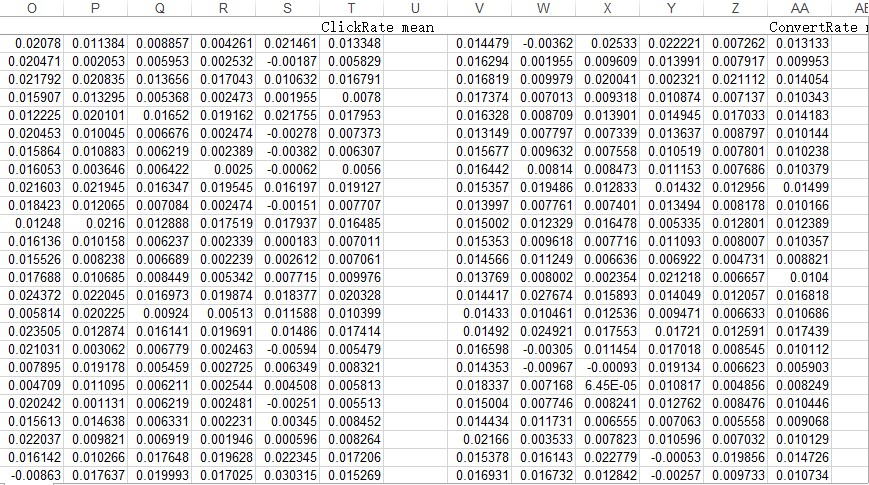
\includegraphics[width=15.00cm]{12.jpg}\\
  \caption{BP Neural Network Result. The error of some numbers is lower than 1\%. }\label{fig12}
\end{figure}


\textbf{It can be seen that some of the predicted data run an accuracy that is higher than 99\%. However, it may overfit the data as the epoch increasing, which finally comes to the XG Boosting Algorithm.}

\subsection{XG Boosting Algorithm}

\textbf{We utilize XG Boosting algorithm to synthesize the three methods above. The basic principle is that it combines several weak classifier into a strong classifier, which ideally suits the problem we are studying. }The basic formula is as the following formula \ref{for33}.

\begin{equation}\label{for33}
L ( \theta ) = \sum _ { i = 1 } ^ { n } l \left( y _ { i } , \widehat { y _ { l } } \right)
\end{equation}

In the formula, $L ( \theta )$ denotes the overall loss of each classifier, $y _ { i }$ denotes each classification function, and $\widehat { y _ { l } }$ is a function of each classifier to reduce the loss. $y _ { 1 }$ denotes the original result of Principal Component Analysis. $x _ { 2 }$ denotes the result of Bayes distinction. $x _ { 3 }$ denotes the original result of BP neural network fitting. For each category in Bayes distinction, we utilize the mid-value of each interval to numerate each category. We divide the click rate into 5 categories, which are 0-0.1, 0.1-0.2, 0.2-0.225, 0.225-0.3, 0.3-0.464, as well as the convert rate into 5 categories, which are 0-0.1, 0.1-0.2, 0.20-0.22, 0.22-0.23, 0.23-0.468. Therefore, we use 0.05, 0.15, 0.2125, 0.2625, and 0.382 to denote the 5 result of the categories. We use 0.05, 0.15, 0.21, 0.225, and 0.349 to denote the 5 result of the categories.

The main theory of BOOST algorithm is as follows. For a complicated issue, it is a better judgment when synthesizing the judgment of each expert than that of a sole expert. For each step, we generate a model accumulate each model to a whole model, which enables us to analyze the problems. Hence, we need to assemble several weak learner into a strong learner by determining the loss functions, $\widehat { y _ { l } }$, to minimalize the error and loss of misjudgment.

We input the predicted result of the three learner into the algorithm as the learning set and the real result as the target goal. We regard test set in the Bayes distinction and BP Neural Network as the testing set. With the help of XG Boosting module in PYTHON, we are able to determine the weight of the three learner to generate the final result. we are able to determine the weight of the three learner to generate the final result. [20]

\textbf{We utilize a formula to measure the error of our estimation, reaping an average score of 9.81 of click rate and 9.74 of convert rate out of 10. }There also exist many data of which the predicted result is exactly the same as the original result, receiving a full score of 10, which shows that this model can successfully reflect the trend. The formula is as the following formula \ref{for34}.

\begin{equation}\label{for34}
S _ { k } = \max \left( 0,10 - 10 \times \left| \frac { \log _ { 10 } \left| \frac { x _ { \text {predict} } } { x _ { r e a l } } \right| } { 5 } \right| \right)
\end{equation}

In the formula, $S _ { k }$ denotes the score of the data, while $x _ { pxedict }$ and $x _ { r e a l }$ respectively denote the predicted value and the real value of the data.

\section{Application}

We use the data which have exactly one zero of each data as the test sets and conduct the 4 modeling process illustrated in part 5 to obtain the final result to show that our models and methods can be applied to a broader range. Figure \ref{fig13} is a part of the final result.

\begin{figure}
  \centering
  % Requires \usepackage{graphicx}
  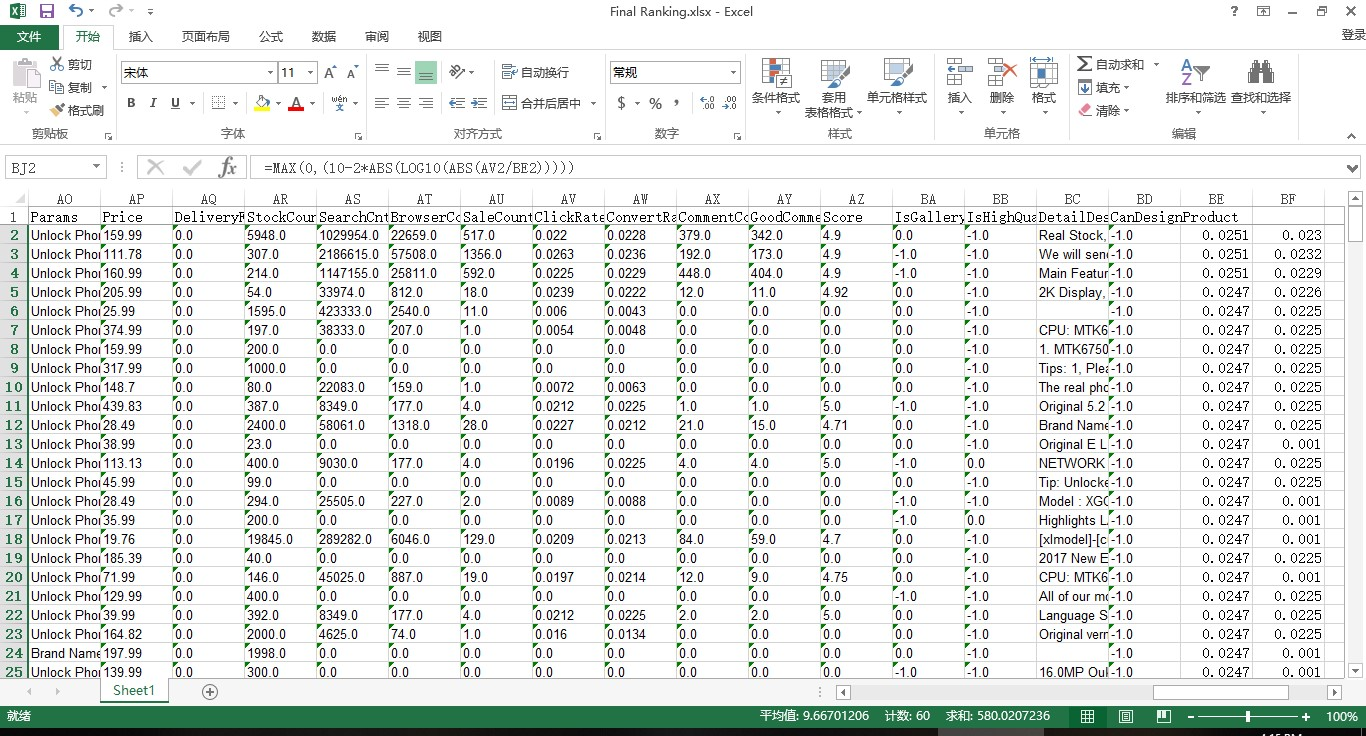
\includegraphics[width=15.00cm]{13.jpg}\\
  \caption{Final Result}\label{fig13}
\end{figure}

\section{Sensitivity Analysis}

Sensitivity analysis is a method of studying and analyzing the sensitivity of the model to changes in system parameters or surrounding conditions. \textbf{In the optimization methods of our team, it can detect the stability of our model, especially when the given data is not accurate.}

In this part, we will mainly discuss the sensitivity of the application part. We divide all the independent variables in two categories: continuous variables and discrete variables.

If the variables are continuous, we do as follow: If we give the test set of the data an increase or a decrease of 1\%, by changing the value of the original data matrix on the program, we discover that the output data of the principal component regression changes precisely 1\%; almost all the results in the Bayes Distinction part have no difference in categories; the majority of the output of BP neural network model fluctuates 1\% approximately.

If the variables are discrete, we conduct the sensitivity analysis one by one, which means each time we only change the data of one properties, remaining the rest of the data unchanged. We change the value of discrete data into adjacent categories, while the top and the bottom data does not change. For instance, when we examine the stability of ROM and we increase the data, we change the data of the phone with 2G into those of 4G, those with 4G into 8G, etc. If the phone has 64G ROM, which is the top, then we remain the data unchanged. The output of the data changes approximately 0.1\%.

\textbf{The output after the change is small enough for us to make a further adjustment. Therefore, it is acceptable in the modeling. }This sensitivity analysis also indicates that our model has universality and can be applied to more situations. For instance, if there is some error in the data, out final result does not vary rapidly correspondingly. Therefore, our model is relatively stable. The data of Sensitivity Analysis can be referred to the appendix part.

\section{Conclusion}
\subsection{Strength and Weakness}

The method we propose in the paper has effectively made up the vacancy and deficiency of the previous evaluating process regarding the sale volume of cell phones, and several main advantages are as the following. For a start, it presents the ranking of the most important individual variables within the cell phone market, the results of which are seldom considered by manufacturers but actually of great significance. Manufacturers can take specific traits of cellphones into consideration, deciding which types or combinations of traits are more profitable to produce and fit the need of their target customers. Furthermore, as the application section in the paper indicates, the process we propose can also be applied to pragmatic purposes. By using the method linked with BP neural network, the process can successfully predict the outcome of the sale volume of cellphones before they are released into the market, and the margin of error is within an acceptable level. Besides the application of the evaluating process in real life, the method itself is also more advanced and comprehensive than that in the previous thesis. For the method of information entropy in data processing and BP neural network in the optimization, they not only fit in the exact needs of the data being processed and the expected outcome, but they are also more precise and reliable, ensuring the credibility of the model as a whole.

Admittedly, there are several shortcomings concerning the whole paper, like for some particular methods including Grey Relational Analysis, the results are not very desirable, and they are not entirely useful for the later optimization. However, considering the techniques being applied as a whole, the advantages obviously outweigh the deficiencies, thus making the modeling reliable for reference and have high practical value.

\subsection{Conclusion}

We have discovered some intriguing and unexpected conclusion throughout the modeling process.
\begin{itemize}
  \item It is the most amusing that phones sold either the best or the worst focus on the highest RAM, ROM, and CPU, which means that these three factors attract the customers a lot. If the mobile manufacturer is willing to enhance the phone specs without adding price, they should consider promoting the RAM, ROM, and CPU for the most priority.
  \item Phones with upper-middle display resolution sell better, while phones with middle and the highest counterparts sell worse. Phones with the lowest and highest recording definition gain better sales. The sellers and manufacturers should not pay much attention to these factors because these factors are less concerned by customers.
  \item For the Highest Camera Resolution and Price, the ones with middle and lower-middle condition sell well, and the ones with upper-middle or the highest equivalents sell experience a tough sell. Maybe the prices are too high for ordinary users to purchase, while the users do not need such high specs on phones. Compared with adding the versatile specs, the manufactures ought to choose lowering down the prices rather.
\end{itemize}
In addition to the specific conclusion and some reasonable explanation, our research also yields significant results in the following four aspects. First, the method concerning Weight determination Technique produces a qualitative analysis of which specific traits in the individual variables promote the sale of the phones the best way. For example, regarding the display resolution, target readers can clearly make out the third category as bringing more profit and contributing more to the sale. The results can be compiled into graphs and thus providing the whole picture in a straightforward way. Besides, Weight determination Technique is an easily accessible method and produces a relatively reliable result.

Second, the quantitative research can be used to rank the factors and determine which elements are the most crucial ones that the manufacturers should take into consideration. The results reflect the tendency of customers towards different types of cell phones, and their preference is carefully studied using information entropy in the data processing. The ranking of individual variables gives the target readers a broader view of which ones are the keys to promoting the sale and lays the stepping stone for the further optimization relating to the different traits in individual variables.

Third, the optimization process allows the determination of specific characteristics that contribute to the highest sales volume. The optimization using Bayes distinction and BP neural network further explores the result in particular details. For example, as for the individual variable like color, it can be analyzed that gold contributes to the highest sale, the fact of which will definitely give the manufacturers more detailed references when making decisions about the production of certain cell phones. For other variables, the same method can be applied, either, yielding valuable insight into specific traits.

Last but not least, the sales volume of the cell phones can be successfully predicted by applying the method in the optimization process, as mentioned in the application section. These methods enable the manufacturers to predict the sale with given characteristics, and according to the sensitivity analysis and data testing, the model is reliable and can be applied for other practical uses.
\newpage
\section{References}
\begin{thebibliography}{}
	\bibitem{1} J. Chevalier, D. Mayzlin. The Effect of Word Of Mouth on Sales: Online Book Review [J]. Working Paper, 2003.12.
	\bibitem{2} Michael D. Smith, Erik Brynjolfsson. Consumer Decision-Making at an Internet Shop bot: Brand Still Matters [J]. The Journal of Industrial Economics, 2001.12(4):541-558.
	\bibitem{3} Jie Z., Jianan Z. Research of promotion's influence to customers' purchasing behaviors [A]. In The 11th National Conference on Psychology [C]. Kaifeng, China, 2007: 278.
	\bibitem{4} Gang D., Zhenyu H. Prediction of customers' purchasing behaviors in the Big Data environment [J]. Modernization of Management, 2015, 1(14): 40-42.
	\bibitem{5} Zhanbo Z., Luping S. and Meng S., Research of comparison between factors in C2C influencing page view and sales volume[J].Journal of Management Science,2013,26(1): 58-67.
	\bibitem{6} Zhihai H., Dandan Z. and Yi Z. An Empirical Study on the Effect of Online Reviews on Product Sales [J]. Journal of Chongqing Technology and Business University (Natural Science Edition), 2015, 12(11): 52-55.
	\bibitem{7} Naicong H., Xu Z., Enjun Z. Grey Relational Analysis of online reputation and sales volume---amovie data as an example [J], Modernization of Management, 2015, 2(10):28-30.
	\bibitem{8} Xiao S. Research of influential factors of online sales based on Grey Relational Analysis [D], Yunnan University of Finance and Economics, Yunnan, 2017.
	\bibitem{9} Youzhi X., Yongfeng G. Competitive Strategy of E-business Sellers on Consumer-to-Consumer Platform: Based on Data from Taobao.com [J], Nankai Business Review, 2012, 15(1): 129-140.
	\bibitem{10} Jingsha F. The Study of Influencing Factors and Index System of C2C Online Shop Sales Volume Based on the Soft Set Theory [D], Chongqing Jiaotong University, Chongqing, 2016.
	\bibitem{11} Wenxuan H. Study on the factors influencing the purchase behavior of Wechat business customers [D], Nanchang University, Nanchang, 2016.
	\bibitem{12} Jiao L. Research on customer purchase behavior analysis system based on Data Mining [J], Time Finance, 2015, 2(2): 320-321.
	\bibitem{13} http://blog.csdn.net/MATLAB\_matlab/article/details/59483185?locationNum=10\&fps=1, MATLAB principal component analysis.
	\bibitem{14} Mingbei C., Gang H., Guoufu Z. Comprehensive evaluation of takeaway website based on AHP method?a?aEleme website as an example [J]. Modern Business, 2015, 12: 57-58.
	\bibitem{15} https://wenku.baidu.com/view/99c8408e6529647d272852cd.html, Interval estimation and linear regression analysis with MATLAB.
	\bibitem{16} Jiang W. Comparative Study of Fisher Discriminant and Mahalanobis Distance Discriminant [J]. Journal of Ningbo Polytechnic, 2017, 21(5); 91-94.
	\bibitem{17} Yimeng F. Analysis of influencing factors of customer purchase behavior in E-commerce [J], Industrial \& Science Tribune, 2014, 13(8): 138-139.
	\bibitem{18} Haiwei W. Yu X., Yalin W.A bivariate hierarchical Bayesian approach to predicting customer purchase behavior [J], Journal of Harbin Engineering University, 2007, 28(8): 949-954.
	\bibitem{19} Wu P. Application of Cigarette Sales Forecasting Based on Neural Network [J], Computer Simulation, 2012, 29(3): 227-230.
	\bibitem{20} https://blog.csdn.net/weixin\_42029738/article/details/81675234, Hand-in writing XG Boost programs.
\end{thebibliography}
\newpage
\section{Acknowledgement}

The division of labor is as follows.

~\\

In the process of writing, Cheng Qian completed the information entropy, the advantages and disadvantages of analysis and conclusion part of the production and writing; Lingwei Cao completed the production and writing of the research background, current research status, research significance and research methods. Zhaoyang Tian completed data processing, grey correlation, principal component analysis and regression, weight determination method, linear regression, distance and bayes discriminant, the BP neural network, the production of XG Boosting algorithm and writing.

~\\

The following is the resume of guidance teachers and team members.

~\\

Hao Wu, associate professor, working from Tsinghua university. Education background: Doctor of applied mathematics, July 2009, Tsinghua university, tutor: professor Shi Jin. Bachelor of mathematics, July 2004, Tsinghua university. Work experience: associate professor in charge, department of mathematical science, Tsinghua university, December 2016-present. Associate professor, department of mathematical science, Tsinghua university, December 2013 to November 2016. Postdoctoral fellow, November 2009 to October 2010, faculty of mathematics, Paul sabati university (top 3 in Toulouse), co-advisor: Prof. Naoufel Ben Abdallah. Member of education committee and China association of industrial and applied mathematics, from December 2016 to now. Main awards: national outstanding doctoral dissertation nomination, academic degrees committee of the state council, 2012. First prize of outstanding young people's thesis, China association of computational mathematics, 2011. Young teachers teaching excellence award, Tsinghua university, 2017. First prize of the 8th Beijing college and university young teachers teaching basic skills competition, Beijing education committee, 2013.

~\\

Dianjun Wang, male, Han nationality, born in September 1960 in Shaanxi Province, China. He received his bachelor��s degree of science in mathematics department of Shaanxi normal university in January 1982. In July 1997, he received his doctor's degree from school of mathematics, Peking University. From August 1997 to July 1999, he was a postdoctoral fellow in mathematics department of Tsinghua university. From August 1999 to December 2006, he served as associate professor and professor of mathematics department of Tsinghua university, and successively served as group leader, deputy secretary of the party committee and secretary of the party committee of the graduate student working group of mathematics department. Since January 2007, he has been the President of the Tsinghua high school. Dianjun Wang has been working in the front-line of teaching and research in the university for a long time. He has given lectures on more than ten courses, including one excellent course from Beijing and one excellent course from Tsinghua university. In the past five years, the teaching evaluation of the main courses taught by Dianjun Wang ranks top 5\% of Tsinghua university. He has completed nearly 10 scientific research projects such as the national natural science foundation of China, published more than 30 academic papers, edited and published two books each, and supervised 2 postdoctoral, 1 doctoral and 5 master's students. He has been awarded ``Linfeng award" for outstanding instructor of Tsinghua university, ``outstanding teaching achievement award of Tsinghua university", ``outstanding teaching achievement award of young teachers of Tsinghua university", ``outstanding teaching achievement award of Beijing", ``education innovative model of Beijing", ``outstanding teacher of Beijing" and other honorary titles.

~\\

Zhaoyang Tian, male, currently studying in Tsinghua High School. I achieved A on each subject in each term and have a strong physique. I scored the top 30 students in school. I was awarded the Honorable Mentioned prize in High School Mathematical Contest in Modeling (HiMCM) in November, 2017. I was awarded the first prize in mathematics, physics, and chemistry of grade 10 in National Mathematics, Physics, and Chemistry Competition for Middle School Students in 2018. I scored 118 and the top 1\% in AMC12 in 2018 and 178 in AIME. I was awarded the first prize (Provincial round) of ``Dengfeng" Cup math modeling competition held by Tsinghua University in March, 2018. I was awarded the second prize (Qualified round) and third prize (National final round) of``Dengfeng" Cup math modeling competition held by Tsinghua University in May, 2018. I scored the top 25\% in algebra test and the top 40\% in geometry test and awarded the second place in calculus test, the second place in power round, the eleventh place in guts round and the ninth place in overall team round in Asdan Math Tournament (AMT) on August, 2018. I participated in the CS Advanced Research Laboratory in Tsinghua High School from September, 2017 and finished the Bring Eyes to The Blind -- A Reminder System for Identifying Traffic Lights project with the help of PYTHON and ARDUINO and Keyword Search and Binary Classification project with the help of URLLIB, TENSORFLOW, JIEBA, and WORDCLOUD module. I was enrolled in Science Talent Program jointly organized by China Association for Science \& Technology (CAST) and Ministry of Education of the P. R. China in 2018, finished Similar News Synthesizing And Positive And Negative Evaluation project and awarded outstanding student of the year.

~\\

Cheng Qian, male, currently studying in Tsinghua High School. I have outstanding academic performances in school, ranking top 5 (top 1\%) in the whole grade. Ranking 2nd in High School Entrance Examination of 2017 in HaiDian District and won the Qidi scholarship. I was awarded the HaiDian District merit student and outstanding student leaders several times. Meanwhile, I participated and organized several school activities as the dais member of the Model United Nations club and the advisor of Shangdi school of Tsinghua High School. I am good at math, and won several first and second award in mathematics, including first prize of Beijing high school mathematic knowledge application competition; first prize of Mathematics competition for grade 10 middle school students in Beijing; second prize of High School Mathematics League. I scored 124 and the top 1\% in AMC12 in 2018 and scored 204 in AIME. Practical experience and reward in mathematical modeling: Honorable Mentioned prize in High School Mathematical Contest in Modeling (HiMCM) in 2017; first Prize in Preliminary contest of Deng Feng Bei mathematical modeling competition; second Prize in quarter-final of Deng Feng Bei mathematical modeling competition; third Prize in final of Deng Feng Bei mathematical modeling competition. Other award: National first prize in Zhong Hua Sheng Tao Bei Middle School Students Writing Competition.

~\\

Lingwei Cao, female, currently studying in Tsinghua High School. I have outstanding academic performances in school, ranking top 20 (top 3\%) in the whole grade. My English performances are especially excellent, with TOEFL score of 115, SAT score of 1540, and AP Calculus score of 5. Academic activities: July, 2018. Attend the ORIC+ Summer Camp (High School) ; July, 2017. Attend Stanford Pre-Collegiate Summer Institution, Logic and Problem-solving course. Awards: March, 2018. First Prize in Preliminary contest of Deng Feng Bei mathematical modeling competition; Second Prize in quarter-final of Deng Feng Bei mathematical modeling competition; Third Prize in final of Deng Feng Bei mathematical modeling competition; January, 2018. Municipal first prize in math subject of National Middle School Students�� Capacity Show; December, 2017. National first prize in 2017 National English Proficiency Competition for Secondary School Students (NEPCS); April, 2018. National third prize in Zhong Hua Sheng Tao Bei Middle School Students Writing Competition; May, 2018. No.8 (Top 10) in Algebra, the second place in power round, the eleventh place in guts round and the ninth place in overall team round in the ASDAN Math Tournament 2018; January, 2018. Honorable Mention in HiMCM; I scored 105 and the top 1\% in AMC12 in 2018 and 178 in AIME.

\newpage
\section{Declaration}
\newpage
\section{Appendix}
%\subsection{}
\appendix


\end{document}
